\chapter{概率分布的分析与优化}
\label{chap:information-theory-and-statistical-geometry}

第一章把随机变量的取值规律写成分布，并建立联合、条件与换测度计算。现在固定两种可能的温度规律：它们可以有相同均值，却有不同尾部；也可以只差一个很小的整体位移，却在某个阈值两侧赋予完全不同的概率。仅凭均值、方差或参数间距，无法回答这些规律在当前任务中是否接近。

本章把概率分布本身作为分析与优化的对象。一张规律的信息量决定记录结果的理想平均描述长度；两张规律的差异则要说明比较的是事件概率、函数期望、质量位置还是对数评分。联合规律与边缘乘积的差异进一步度量变量之间的依赖。允许近似还原时，描述长度还须与重构误差一起考虑，不能只由无失真熵决定。

这些分析也为分布选择建立条件。逼近分布时，先说明何种探针或距离趋于一致，以及质量是否逃向远处；固定评价函数时，再把分布差异转成期望变化的界。收益、矩条件、候选表示或边缘约束确定可行分布，局部几何则决定参数更新的分布步长。有限样本能否估准这些量、能否辨认候选规律，留到第~\ref{chap:statistical-inference}章讨论；这里先研究给定概率规律时成立的关系。

除编码处显式使用\(\log_2\)外，本章的\(\log\)均为自然对数；相应的信息量以nat计。
以二为底计算的信息量以bit计，\(1\ \mathrm{bit}=(\log2)\ \mathrm{nat}\)。

\section{观测的信息量}
\label{sec:information-uncertainty-prediction}

设一串记录按已知规律产生，常见结果会反复出现。给常见结果短码、罕见结果长码，可以降低每条记录的平均描述长度；这个平均由出现概率决定。若另一个变量已经被观察，还可以只描述剩余的不确定部分。离散结果能够直接对应码字，连续结果则要同时规定记录精度。

\Needspace{7\baselineskip}
\subsection{离散观测的信息量}
\label{sec:information-entropy}

\subsubsection{无条件观测的平均信息量}
\label{sec:information-unconditional-information}

设结果\(x\)的发生概率为\(p(x)>0\)，我们希望用一个数表示它的“意外程度”：看到几乎必然发生的结果并不意外，看到罕见结果才带来大量新信息。把发生概率为\(p\)的结果的描述代价记为\(c(p)\)，先从两个最朴素的要求确定它的形式。两个独立结果的发生概率相乘，
而同时描述它们的代价应当相加——无论先描述哪一个，合起来的字数都应是两段字数之和，因此要求
\[
  c(pq)=c(p)+c(q),\qquad 0<p,q\leq1.
\]
再要求\(c\)连续，且概率越小代价越大。令\(u=-\log p\)，
函数\(b(u)=c(e^{-u})\)便在\(u\geq0\)上满足\(b(u+v)=b(u)+b(v)\)。
连续的可加函数为线性函数；上述单调要求使其斜率为正，因而
\(c(p)=-a\log p\)，其中\(a>0\)。系数\(a\)只改变信息量的单位。
按本章的自然对数约定取\(a=1\)，便得到\term{自信息}（self-information）
\(-\log p(x)\)：罕见结果的自信息更大。它描述单次结果，尚未对所有可能结果平均。

\begin{definition}[离散熵]
\label{def:information-discrete-entropy}
设离散随机变量\(X\)取值于有限或可数字母表\(\mathcal X\)，质量函数为\(p\)。
其\term{熵}（entropy）是自信息的平均：
\begin{equation}
  H(X)=-\sum_{x\in\mathcal X}p(x)\log p(x)
      =\mathbb E[-\log p(X)].
  \label{eq:information-discrete-entropy}
\end{equation}
约定\(0\log0=0\)：概率为零的结果永远不会出现，对平均描述长度没有贡献，取极限\(p\log p\to0\)（\(p\downarrow0\)）也得到同一数值。这是非负扩展值求和，可以为\(+\infty\)。
熵有限的条件可写为
\[
  \sum_xp(x)|\log p(x)|<\infty.
\]
\end{definition}

常量没有待区分的结果，熵为零；\(m\)个等概率结果的熵为\(\log m\)。
例如\(X\sim\operatorname{Bernoulli}(1/4)\)时，
\[
  H(X)=-\tfrac14\log\tfrac14-\tfrac34\log\tfrac34
       \approx0.5623\ \mathrm{nat}\approx0.8113\ \mathrm{bit}.
\]
结果\(1\)的自信息为\(2\) bit，但它只占四分之一的发生概率，所以平均值不到一位。

把同一个定义用在字母表大小相同而分布不同的两个变量上，可以看清熵比较的到底是什么。
设\(X\)在四个结果上均匀分布，\(Y\)的分布为\((0.7,0.2,0.06,0.04)\)，则
\[
\begin{aligned}
  H(X)&=2\ \mathrm{bit},\\
  H(Y)&\approx0.7\times0.515+0.2\times2.322\\
      &\quad+0.06\times4.059+0.04\times4.644\\
      &\approx1.254\ \mathrm{bit}.
\end{aligned}
\]
两者字母表大小相同，熵却不相等。熵并不衡量“有多少种可能”，而是衡量按现有分布
把结果平均区分开需要多少信息：\(Y\)以\(0.7\)的概率取第一个结果，
概率质量集中在少数结果上，平均描述所需的信息就较少。若\(Y\)的概率质量再集中一些，
例如分布\((0.97,0.01,0.01,0.01)\)，熵降到
约\(0.242\) bit。反过来，合并结果会丢失一部分不确定性：把\(Y\)的后三个结果合并为一个，
得到\((0.7,0.3)\)，熵约\(0.881\) bit，低于原来的\(1.254\) bit。被合并掉的那部分
内部差异不再计入，得到的分布也对应另一个变量。

\subsubsection{条件观测的剩余信息量}
\label{sec:information-remaining-information}

现在考虑先观察一个相关变量，再描述另一个变量。若发送者和接收者都知道\(Y=y\)，双方共享这一信息，需要描述的就只是在这个已知值下\(X\)还剩多少不确定，即条件分布\(p(x\mid y)\)，
而不是重新描述整个\(X\)。例如先告诉接收者当天是工作日还是周末，再描述路况：知道“周末”以后，拥堵已经不太意外，剩余描述应当按这一条件下的概率重新计算。前章的条件分布使这一点可以逐个条件值计算。

\begin{definition}[离散条件熵]
\label{def:information-conditional-entropy}
对离散随机变量\(X,Y\)，在\(p(y)>0\)处令
\(H(X\mid Y=y)=-\sum_xp(x\mid y)\log p(x\mid y)\)。
\term{条件熵}（conditional entropy）定义为这些剩余信息量的平均：
\begin{equation}
  H(X\mid Y)=\sum_yp(y)H(X\mid Y=y)
           =-\sum_{x,y}p(x,y)\log p(x\mid y).
  \label{eq:information-conditional-entropy}
\end{equation}
零质量条件值可以任意指定条件分布，贡献为零；结果允许为\(+\infty\)。
\end{definition}

在联合质量为正的点，\(p(x,y)=p(y)p(x\mid y)\)。
对负对数取期望得到
\[
\begin{aligned}
  H(X,Y)
  &=-\sum_{x,y}p(x,y)\log p(y)
    -\sum_{x,y}p(x,y)\log p(x\mid y)\\
  &=H(Y)+H(X\mid Y).
\end{aligned}
\]
这些项非负，非负求和换序保证等式在扩展值意义下也成立。
反复分解给出联合熵的链式法则：
\begin{equation}
  H(X_1,\ldots,X_n)
  =\sum_{i=1}^nH(X_i\mid X_1,\ldots,X_{i-1}).
  \label{eq:information-entropy-chain-rule}
\end{equation}
链式法则不要求独立；独立时各条件熵才可换成无条件熵。
若要移项写成熵之差，必须确认相应熵有限，不能计算\(\infty-\infty\)。

\begin{example}[一次带噪二元观测]
\label{ex:information-binary-channel}
令\(X\)在\(\{0,1\}\)上均匀，观测\(Y=X\oplus N\)，其中\(\oplus\)为异或，
\(N\sim\operatorname{Bernoulli}(\varepsilon)\)独立于\(X\)，
\(0\leq\varepsilon\leq1/2\)。对每个\(y\)，
\[
  P(X=y\mid Y=y)=1-\varepsilon,\qquad
  P(X=1-y\mid Y=y)=\varepsilon.
\]
定义二元熵函数
\(H_{\mathrm b}(u)=-u\log u-(1-u)\log(1-u)\)，端点沿用零项约定。
于是\(H(X)=\log2\)、\(H(X\mid Y)=H_{\mathrm b}(\varepsilon)\)。
当\(\varepsilon=1/4\)时，观测后剩余\(0.5623\) nat，
比观测前少\(0.1308\) nat；无噪声时没有剩余不确定性，
公平翻转时则仍剩全部\(\log2\) nat。
\end{example}

这里计算的是条件分布下的平均剩余量，不是每次观测都能准确恢复的保证。
减少部分怎样描述两个变量的关系，将在第~\ref{sec:information-mutual-relations}节
用一般测度上的分布比较给出定义，并画出条件熵与互信息随噪声变化的曲线。

\subsection{连续观测的信息量}
\label{sec:information-continuous-information}

\paragraph{记录精度对编码长度的影响}
连续结果若要求无限精度，单次记录通常不能用有限比特无失真描述：实数轴上任意非退化区间内都有不可数多个取值，而所有有限二进串也只有可数多个，无法把这些取值全部一一区分。实际记录总要规定精度，例如温度只报到\(0.1\)度。可以先把实轴分成宽度\(\Delta\)的小格，每个读数只记录它落入哪一格；在密度足够规则时，
格子概率近似\(p(x)\Delta\)。把量化后的离散变量记为\(X_\Delta\)，对这些格子计算的离散熵近似为
\[
 H(X_\Delta)\approx-\int p(x)\log p(x)\,\mathrm dx-\log\Delta,
\]
单位仍为nat。精度代价\(-\log\Delta\)随格子细化而增大，余下的密度项才是微分熵；格子宽度与密度须使用同一坐标单位。
若要转换为二进制码长，须先除以\(\log2\)。在量化熵有限时，定理~\ref{thm:information-source-coding-bound}还将给出可实现前缀码的平均长度与\(H(X_\Delta)/\log2\)相差不到一比特，不能把熵的近似直接当成任意编码的精确长度。这里仅解释量化与精度的关系，不主张该渐近式对任意密度成立。

\paragraph{基于概率密度的微分熵}
\begin{definition}[微分熵]
\label{def:information-differential-entropy}
固定参考测度\(\mu\)。若\(P\ll\mu\)、\(p=\mathrm dP/\mathrm d\mu\)，且
\(\mathbb E_P|\log p(X)|<\infty\)，定义相对于\(\mu\)的熵
\[
  h_\mu(P)=-\int p\log p\,\mathrm d\mu.
\]
在\(\mathbb R^d\)上取Lebesgue测度时，称为\term{微分熵}
（differential entropy），简记为\(h(\bm X)\)。
\end{definition}

指定参考测度是定义的一部分。若换成\(\mu'=a\mu\)，其中\(a>0\)，
密度变为\(p/a\)，故\(h_{\mu'}(P)=h_\mu(P)+\log a\)。
与离散质量不同，密度可能大于一，其负对数也可能为负。
例如\(X\)在\([0,1/2]\)上均匀时密度为\(2\)，
\(h(X)=-\log2\)。这不是负的码长，而是脱离指定精度后留下的密度项。

图~\ref{fig:information-quantization-entropy}进一步固定坐标单位，只改变记录精度。对\([0,1]\)上的均匀变量划分\(n\)个等宽格时，每格概率恰为\(1/n\)，所以量化熵精确等于\(\log n\)，而微分熵保持为零。由格数增加而产生的离散信息量，不能用不含分辨率的微分熵直接替代。

\begin{figure}[htbp]
  \centering
  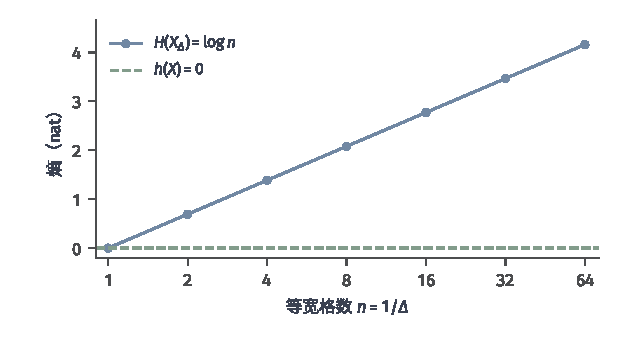
\includegraphics[width=105mm]{figures/00-shared/mathematical-preliminaries-lower/01-random-variables-distributions-and-causality/matplotlib/information-quantization-entropy/figure.pdf}
  \caption{均匀分布的量化熵与记录分辨率。取\(X\sim\operatorname{Unif}[0,1]\)，格宽\(\Delta=1/n\)，蓝线标记\(n=1,2,4,\ldots,64\)时的精确离散熵\(H(X_\Delta)=\log n\)，绿虚线为\(h(X)=0\)，单位均为nat。横轴为以\(2\)为底的对数刻度，连接线只引导比较所列格数。}
  \label{fig:information-quantization-entropy}
\end{figure}

\paragraph{变量变换对微分熵的影响}
只改变数值尺度，也会改变微分熵。沿用上面的均匀变量，令\(Y=2X\)，
则\(Y\)在\([0,1]\)上均匀，密度为\(1\)，所以\(h(Y)=0\)，比\(h(X)\)增加\(\log2\)。
若\(X\)和\(Y\)是同一物理量在不同单位下的数值，这次换算并没有增加观测信息，
却改变了微分熵。因此，微分熵的数值需要连同坐标单位和记录精度一起理解。

为了把这个尺度例子推广到一般坐标变化，设\(\bm X\)具有Lebesgue密度\(p_{\bm X}\)，且
\(\mathbb E|\log p_{\bm X}(\bm X)|<\infty\)。
令\(g:\mathbb R^d\to\mathbb R^d\)为\(C^1\)微分同胚，
\(\bm Y=g(\bm X)\)，且
\(\mathbb E|\log|\det\bm J_g(\bm X)||<\infty\)。
由前章密度换元公式，
\(p_{\bm Y}(g(\bm x))=p_{\bm X}(\bm x)/|\det\bm J_g(\bm x)|\)。
取负对数并按\(\bm X\)平均，便得到
\begin{equation}
  h(\bm Y)=h(\bm X)+
  \mathbb E\log|\det\bm J_g(\bm X)|.
  \label{eq:information-differential-entropy-transform}
\end{equation}
特别地，对可逆矩阵\(\bm A\)，
\(h(\bm A\bm X+\bm b)=h(\bm X)+\log|\det\bm A|\)。
刚才的\(Y=2X\)就是一维变换\(g(x)=2x\)的特例，导数为\(2\)，所以熵增加\(\log2\)。
若长度的米数为\(X\)，厘米数为\(Y=100X\)，换元公式则给出
\[
  p_Y(y)=\frac1{100}p_X(y/100),\qquad h(Y)=h(X)+\log100.
\]
数值区间扩大\(100\)倍，密度高度相应缩小为原来的\(1/100\)。
同一物理测量精度在厘米中的数值也要乘以\(100\)，这次单位换算没有新增观测信息。
若要比较两张分布而不受共同坐标换元影响，可以使用下一节的KL散度：
其对数密度比中的共同Jacobian因子会相消，积分得到的比较量因而保持不变。

\subsection{基于概率模型的无失真编码}
\label{sec:information-lossless-coding}

熵还可以用来判断编码的平均长度能降低到什么程度。回到概率为\((0.7,0.2,0.06,0.04)\)的四符号变量\(Y\)，把理想码长向上取整，
取\(\ell(x)=\lceil-\log_2p(x)\rceil\)，得到码长\(1,3,5,5\)，平均为
\(0.7+0.6+0.3+0.2=1.8\) bit，与\(H(Y)\)相差不到一位。
若忽略各结果的出现概率，统一使用两位码，常见结果也要支付两位，平均码长便增加到\(2\) bit。
不过，指定各个码长还不够，码字串接后必须能够解码。
下面先说明可解码性对码长的限制，再证明取整码长可以实现，并且其平均长度与熵相差不到一位。

二进制前缀码（prefix code）要求任何码字都不是另一个码字的前缀，
因此串接后可以逐个解析。码字\(0,10,11\)满足这一要求，\(0,01\)则不满足。
若码长为非负整数\(\ell(x)\)，把长度为\(\ell\)的码字看成二叉树深度\(\ell\)
的节点，它占据的后代比例是\(2^{-\ell}\)。前缀码所占的后代不能重叠，故
\[
  \sum_x2^{-\ell(x)}\leq1.
\]
这就是Kraft约束。理想实数码长\(-\log_2p(x)\)恰好使总和为一，
实际码长则还要满足整数约束\scite{math-cover2006information}

\begin{theorem}[无失真前缀码的平均长度界]
\label{thm:information-source-coding-bound}
对熵有限的质量函数\(p\)，任意满足Kraft约束的二进制码长均满足
\[
  \mathbb E\ell(X)\geq H(X)/\log2.
\]
在有效字母表\(\mathcal X_+=\{x:p(x)>0\}\)上，
\(\ell(x)=\lceil-\log_2p(x)\rceil\)可由前缀码实现，并且
\[
  \mathbb E\ell(X)<H(X)/\log2+1.
\]
\end{theorem}
\begin{proof}
若平均码长无限，下界直接成立。否则令
\(K=\sum_x2^{-\ell(x)}\in(0,1]\)、\(q(x)=2^{-\ell(x)}/K\)。
由\(-\log u\geq1-u\)，在\(p>0\)的点上求和得到
\[
  \sum_xp(x)\log\frac{p(x)}{q(x)}
  \geq1-\sum_{x:p(x)>0}q(x)\geq0.
\]
所以
\[
  0\leq-H(X)+(\log2)\mathbb E\ell(X)+\log K.
\]
因\(\log K\leq0\)，移项即得下界。这里直接证明所需的对数不等式，
没有预先使用后文才定义的KL。

对取整码长，\(2^{-\ell(x)}\leq p(x)\)，故满足Kraft约束。
按码长非降排列有效字母表，依次在\([0,1)\)放置长度\(2^{-\ell(x)}\)
的半开二进区间。此前区间长度都是当前长度的整数倍，因此新左端点仍与当前
二进网格对齐；总长度不超过一，区间都能放下。以左端点的前\(\ell(x)\)个
二进位为码字。若一个码字是另一个的前缀，相应二进区间便会嵌套，
与区间互不相交矛盾。这个构造也适用于可数字母表，因为每个有限码长下只能有有限个码字。
再对\(\lceil a\rceil<a+1\)平均，得到严格上界。
\end{proof}

\subsubsection{Shannon编码}
\label{sec:information-shannon-coding}
\term{Shannon编码}（Shannon coding）把各符号的理想码长向上取整，再按Kraft约束实现前缀码。上一定理中的构造说明它为何可解码，也说明取整代价每个编码块不到一比特。对刚才的四符号概率，可以选取码字\(0,100,10100,10101\)，码长依次为\(1,3,5,5\)，平均长度为\(1.8\) bit；其二进区间互不相交，因而没有一个码字是另一个的前缀。

Bernoulli例子的两个有效结果都必须使用至少一位，逐符号码长为\(1\) bit；
与\(0.8113\) bit的差来自整数限制。对独立的\(n\)个结果一起编码，
块熵为\(nH(X)\)，每符号冗余可小于\(1/n\) bit。零质量符号已从有效字母表删除；
若也必须传输它们，要额外留出码空间。只有一个有效符号时，上述约定允许空码字，
并假定符号个数已知。允许重建失真则是另一任务，码长还依赖失真准则，
不能仅由熵决定。

\subsubsection{Huffman编码}
\label{sec:information-huffman-coding}
逐个理想码长取整容易实现，却未必使整数码长的平均值最小。对有限有效字母表，\term{Huffman编码}（Huffman coding）每次合并概率最小的两个符号，把它们看作一个概率相加的新符号；仅剩一个节点后，从根到叶的左右分支依次赋\(0,1\)，就得到原符号的前缀码\scite{vision-huffman1952}。

这条合并规则可以由最优树的结构证明。给定满二叉前缀树，若较大概率处在更深叶子，交换它与较小概率只会减小或保持平均码长。于是可选择一棵最优树，使概率最小的两个符号位于最深的一对兄弟叶子。把这对叶子缩成其父节点，平均码长恰减少这两个概率之和；若缩成后的树不是约化字母表的最优树，替换成更优树便会改进原树，与最优性矛盾。反复应用这一论证，就得到合并算法的最优性；有并列概率时，最优树可以不唯一。

对同一概率\((0.7,0.2,0.06,0.04)\)，依次合并\(0.04+0.06=0.10\)、\(0.10+0.20=0.30\)、\(0.30+0.70=1\)。一组码字为\(0,10,110,111\)，平均码长为\(0.7+0.4+0.18+0.12=1.4\) bit，低于前述Shannon码的\(1.8\) bit。最优性限定在这个已知符号分布的逐符号二进制前缀码；它不表示任何序列编码都至少需要\(1.4\) bit每符号。

\subsubsection{算术编码}
\label{sec:information-arithmetic-coding}
逐符号前缀码仍为每个符号单独付出整数位数。\term{算术编码}（arithmetic coding）改为用一个不断缩小的区间描述整段符号序列：起始区间为\([0,1)\)，按当前符号概率将它分成相应比例的子区间，观察一个符号就保留对应子区间，再在其内部继续划分。编码者与解码者共享相同的符号顺序、概率模型及终止规则，便能从最终区间内的二进描述逐步恢复原序列\scite{math-witten1987arithmetic}。

若当前区间为\([a,b)\)，符号\(x\)的累计概率左右端点为\(C_-(x),C_+(x)\)，更新为
\[
 [a+(b-a)C_-(x),\ a+(b-a)C_+(x)).
\]
使用条件概率\(q(x_t\mid x_{<t})\)时，\(n\)步后的区间宽度恰为
\(q(x_{1:n})=\prod_{t=1}^nq(x_t\mid x_{<t})\)。整数限制因此作用于整段序列，而不是每个符号。以\(P(A)=3/4,P(B)=1/4\)且按\(A,B\)排序为例，序列\(AB\)依次得到区间\([0,3/4)\)和\([9/16,3/4)\)。二进区间\([10/16,11/16)\)位于其中，发送其前缀\(1010\)并告知序列长度即可无歧义还原；这个短例只展示机制，不声称已达到最短码长。

任意宽度为\(w>0\)的半开区间都包含一个长度至少\(w/4\)的二进网格小格：选择\(m\)使\(2^{-m}\leq w/2<2^{-m+1}\)，区间内至少容纳一个完整的\(2^{-m}\)小格。因此最终码长可取为小于\(-\log_2q(x_{1:n})+2\)的整数，前提是块长或终止信息已另行约定。模型正确且熵有限时，平均每符号码长接近块熵除以\(n\log2\)。实际有限精度实现还要处理区间缩放、舍入和模型传输；错误模型的代价由下一节的交叉熵与KL衡量。

\section{概率分布的差异}
\label{sec:information-distribution-relations}
\label{sec:information-comparison-identification}
\label{sec:information-distribution-discrepancies}

下面始终比较同一空间上的两张分布\(P,Q\)。事件概率差关注发生与否，核均值差关注一组特征的平均，搬运成本关注质量位置，对数评分关注为真实结果分配的概率。这些观察口径各有尺度与使用条件，最后再比较它们之间能否相互控制。

\subsection{概率权重的差异}
\label{sec:information-probability-discrepancy}

报警规则由一个事件\(A\)指定，观测落入\(A\)时就触发报警。
若尚未决定具体规则，可以问所有事件中，哪一个的发生概率改变最多。
若每个事件在两种规律下的概率都接近，那么任何基于这次观测的报警规则，
在两种规律下的触发概率也接近。下面的总变差距离取这些概率差的上确界，
统一控制所有可测报警规则；它与最优检验错误的精确关系将在第~\ref{sec:information-two-candidates}节推导。

\begin{definition}[总变差距离]
\label{def:information-total-variation}
同一可测空间上概率测度的\term{总变差距离}（total variation distance, TV）为
\begin{equation}
  d_{\mathrm{TV}}(P,Q)=\sup_A|P(A)-Q(A)|,
  \label{eq:information-total-variation}
\end{equation}
其中上确界遍历全部可测事件。
\end{definition}

取共同支配测度\(\mu\)，密度为\(p,q\)。
由于\(\int(p-q)\,\mathrm d\mu=0\)，正部与负部积分相等。
任意事件上的差不超过正部积分，而\(A^\star=\{p\geq q\}\)达到该值，所以
\begin{equation}
  d_{\mathrm{TV}}(P,Q)=\tfrac12\int|p-q|\,\mathrm d\mu
   =P(A^\star)-Q(A^\star).
  \label{eq:information-tv-density}
\end{equation}
对\(|f|\leq1\)，积分的绝对值不超过\(\int|p-q|\)；
取\(f=2\mathbb I_{A^\star}-1\)达到上界，故
\begin{equation}
  2d_{\mathrm{TV}}(P,Q)
   =\sup_{\|f\|_\infty\leq1}|\mathbb E_Pf-\mathbb E_Qf|.
  \label{eq:information-tv-dual}
\end{equation}
若\(0\leq f\leq1\)，令\(g=2f-1\)，相应上确界则恰为\(d_{\mathrm{TV}}\)。
事件指标给出取等号的函数。这两个常数的差别来自值域宽度，不是定义冲突。

总变差只比较事件概率，用密度差的绝对值积分得到；它对概率从哪里搬到哪里并不敏感。换一种思路，可以先把概率向量变成几何对象，再直接量两个对象之间的距离。比较二点分布\((1,0)\)与\((1/2,1/2)\)时，可以先把两个概率向量的每个分量开平方，得到
\((1,0)\)与\((1/\sqrt2,1/\sqrt2)\)。两个新向量长度都为\(1\)，因此能够用同一单位球面上的欧氏距离比较形状。
连续情形也一样：密度满足\(\int p\,\mathrm d\mu=1\)，所以\(\|\sqrt p\|_{L^2(\mu)}=1\)。
直接使用\(p\)未必有有限的\(L^2\)范数；开平方则把每个概率密度都放到同一个Hilbert空间单位球面上，于是“两张分布差多远”就转化为球面上两点的距离。

\begin{definition}[Hellinger距离]
\label{def:information-hellinger-distance}
在共同支配测度\(\mu\)下，定义平方\term{Hellinger距离}为
\begin{equation}
  d_{\mathrm H}^2(P,Q)=\tfrac12\int(\sqrt p-\sqrt q)^2\,\mathrm d\mu
   =1-\int\sqrt{pq}\,\mathrm d\mu,
  \label{eq:information-hellinger}
\end{equation}
距离本身为其非负平方根。
\end{definition}
更换共同支配测度时，两个平方根都乘以同一密度因子的平方根，
积分换元后不变。对三个分布可统一使用其和作支配测度，
从\(L^2\)三角不等式得到\(d_{\mathrm H}\)的三角不等式。
利用
\(|p-q|=|\sqrt p-\sqrt q|(\sqrt p+\sqrt q)\)，有
\[
  d_{\mathrm H}^2(P,Q)\leq d_{\mathrm{TV}}(P,Q)
  \leq\sqrt2\,d_{\mathrm H}(P,Q).
\]
左侧用\(\sqrt p+\sqrt q\geq|\sqrt p-\sqrt q|\)；
右侧用Cauchy--Schwarz以及
\(\int(\sqrt p+\sqrt q)^2\,\mathrm d\mu\leq4\)。

\paragraph{基于密度重叠的Bhattacharyya比较}
若只记录两个密度的重叠程度，可以取出Hellinger式中的平方根内积，记为Bhattacharyya系数：
\[
  \operatorname{BC}(P,Q)=\int\sqrt{pq}\,\mathrm d\mu.
\]
它是平方根密度的内积，取值于\([0,1]\)；值越大表示重叠越多。相应的Bhattacharyya差异定义为\(D_{\mathrm B}(P,Q)=-\log\operatorname{BC}(P,Q)\)，零系数对应无穷。它满足\(d_{\mathrm H}^2=1-e^{-D_{\mathrm B}}\)，但对数变换不保留三角不等式，不能因此把它当作度量。

对正定协方差的两个高斯分布，令\(\overline{\bm\Sigma}=(\bm\Sigma_1+\bm\Sigma_2)/2\)、\(\bm\delta=\bm m_1-\bm m_2\)，配方并积分高斯密度的平方根乘积得到
\begin{equation}
 D_{\mathrm B}(P,Q)
 =\frac18\bm\delta^\top\overline{\bm\Sigma}^{-1}\bm\delta
 +\frac12\log\frac{\det\overline{\bm\Sigma}}
 {\sqrt{\det\bm\Sigma_1\det\bm\Sigma_2}}.
 \label{eq:information-gaussian-bhattacharyya}
\end{equation}
两个项分别来自均值错位和协方差形状的不一致；详细的指数族表达可见Nielsen与Boltz\scite{math-nielsen2011bhattacharyya}。同协方差时只剩第一项，例如\(\mathcal N(0,1)\)与\(\mathcal N(h,1)\)给出\(D_{\mathrm B}=h^2/8\)。对\(h=2\)，两段位移的差异相加为\(1/8+1/8=1/4\)，却小于总位移的\(1/2\)，直接说明三角不等式失败。协方差奇异时原空间没有这些Lebesgue密度，须回到共同支配测度下的系数定义，不能直接套用逆矩阵和行列式。

\subsection{基于核均值的分布差异}
\label{sec:information-test-functions}

同一均值可以对应不同分布，因为单个读数只保留一项平均。若将每个取值映为一组丰富特征，再比较所有特征的平均，就有机会保留更多分布信息。核方法用\(k(x,\cdot)\)作为特征，并把比较范围限制在核所定义的函数空间单位球；这个尺度限制防止任意放大函数而使差异无穷。

\begin{definition}[最大均值差异]
\label{def:information-mmd}
设\(\mathcal H\)为再生核Hilbert空间，核\(k\)可测，且
\[
  \mathbb E_P\sqrt{k(X,X)}<\infty,\qquad
  \mathbb E_Q\sqrt{k(Y,Y)}<\infty.
\]
\term{最大均值差异}（maximum mean discrepancy, MMD）定义为
\[
  \operatorname{MMD}(P,Q)=
   \sup_{\|f\|_{\mathcal H}\leq1}|\mathbb E_Pf-\mathbb E_Qf|.
\]
\end{definition}

这里的\(f\)不再是任意有界函数，而是核\(k\)所确定的函数空间中的元素；单位球约束防止尺度任意放大。再生性质给出
\(|f(x)|\leq\|f\|_{\mathcal H}\sqrt{k(x,x)}\)，
所以\(f\mapsto\mathbb E_Pf\)是有界线性泛函。
Riesz表示定理保证存在唯一代表元\(\bm\mu_P\in\mathcal H\)，使
\(\mathbb E_Pf=\langle f,\bm\mu_P\rangle_{\mathcal H}\)。
这就是核均值（kernel mean embedding）：它是\(\mathcal H\)中的一个元素，
把分布\(P\)对每个\(f\in\mathcal H\)的期望统一表示为与该元素的内积。
不必预先假定Hilbert值积分存在；记号\(\mathbb E_Pk(X,\cdot)\)可由这个代表元解释。
相关的再生核Hilbert空间、有界线性泛函与Riesz表示工具可参考
\BookChapterRef{chap:rkhs}{卷二“再生核Hilbert空间”章}。
对\(Q\)同理，于是
\[
  \operatorname{MMD}(P,Q)
  =\sup_{\|f\|_{\mathcal H}\leq1}
     |\langle f,\bm\mu_P-\bm\mu_Q\rangle|
  =\|\bm\mu_P-\bm\mu_Q\|_{\mathcal H}.
\]
若\(\bm\mu_P-\bm\mu_Q\neq\bm0\)，取
\(f=(\bm\mu_P-\bm\mu_Q)/\|\bm\mu_P-\bm\mu_Q\|_{\mathcal H}\)
便达到上确界。对可测有界核，所需可积条件自动满足。

把分布映成核均值会不会丢掉信息？普通均值相同的两张分布可以完全不同，核均值也只有在所选核足以区分候选分布时才避免这个问题。下面的条件要求不同分布不能被映到同一个核均值；它决定零MMD能否被解释为同分布。
\begin{definition}[核的特征性]
\label{def:information-characteristic-kernel}
在核均值均存在的指定分布类\(\mathcal P\)上，若
\(\bm\mu_P=\bm\mu_Q\)蕴含\(P=Q\)，即核均值映射为单射，
则称核\(k\)在\(\mathcal P\)上具有特征性（characteristic）。
\end{definition}

零MMD能否推出同分布，取决于这个条件。取同一对分布
\(P=\delta_0\)、\(Q=(\delta_{-1}+\delta_1)/2\)。
线性核\(k(x,y)=xy\)只比较普通均值，故MMD为零，
但\(P(\{0\})=1\)、\(Q(\{0\})=0\)。
改用高斯核\(k(x,y)=e^{-(x-y)^2/2}\)，展开核均值范数并用独立副本可得
\[
\begin{aligned}
  \operatorname{MMD}^2(P,Q)
  &=\mathbb E_{P\otimes P}k+\mathbb E_{Q\otimes Q}k
      -2\mathbb E_{P\otimes Q}k\\
  &=\tfrac32+\tfrac12e^{-2}-2e^{-1/2}>0.
\end{aligned}
\]
矩条件通过\(|k(x,y)|\leq\sqrt{k(x,x)k(y,y)}\)保证展开中的积分可交换。
图~\ref{fig:information-kernel-distinguishability}固定这两个分布，只改变核。
该算例证明高斯核能区分这一对对象，不代替整个分布类上的特征性证明。
\begin{figure*}[htbp]
  \centering
  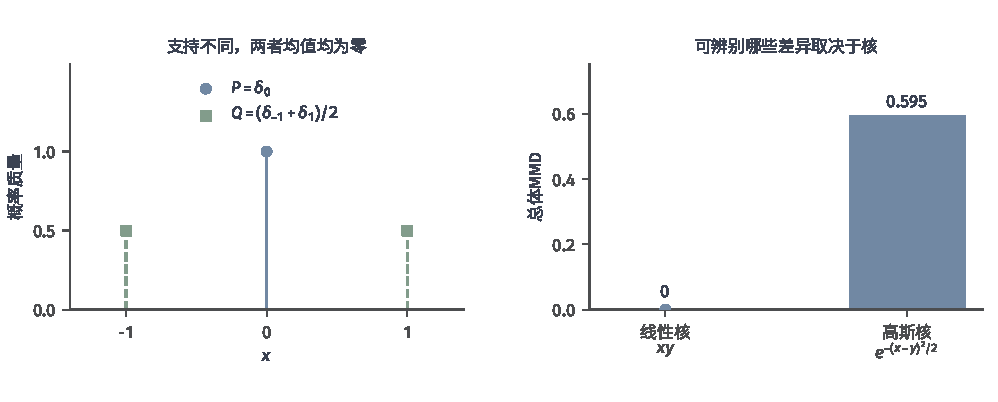
\includegraphics[width=\linewidth]{figures/00-shared/mathematical-preliminaries-lower/01-random-variables-distributions-and-causality/matplotlib/information-kernel-distinguishability/figure.pdf}
  \caption{同均值分布在不同核下的MMD（解析式教学图）。左图为\(P=\delta_0\)与\(Q=(\delta_{-1}+\delta_1)/2\)，右图按精确总体期望计算：线性核给出零，高斯核给出约\(0.595\)。没有使用有限样本估计；差别来自测试函数类。}
  \label{fig:information-kernel-distinguishability}
\end{figure*}

\subsection{质量位置的差异}
\label{sec:information-optimal-transport}

两个不同位置上的点质量没有重叠，TV因而始终为一。若结果是温度读数，把全部质量移动\(0.01\)度与移动\(10\)度却有不同意义。事件概率差没有记录这两个位置之间的距离，质量位置的比较需要使用样本空间本身的几何。\term{最优传输}
（optimal transport, OT）寻找保持两边概率不变的最便宜配对
\scite{math-villani2009transport}。可以把它想成一批仓库向一批门店运货：仓库\(x\)有\(P\)比例的货，门店\(y\)需要\(Q\)比例的货，从\(x\)运一单位到\(y\)的运费是\(c(x,y)\)；怎么安排每对“仓库—门店”之间运多少，才能既不改变各仓库的出货总量和各门店的进货总量，又使总运费最小。

\begin{definition}[耦合]
\label{def:information-coupling}
给定\((\mathcal X,\mathcal A)\)、\((\mathcal Y,\mathcal B)\)上的概率测度\(P,Q\)，
其\term{耦合}（coupling）是乘积空间上的概率测度\(\gamma\)，对所有
\(A\in\mathcal A\)、\(B\in\mathcal B\)满足
\[
  \gamma(A\times\mathcal Y)=P(A),\qquad
  \gamma(\mathcal X\times B)=Q(B).
\]
全体耦合记为\(\Pi(P,Q)\)。
\end{definition}
耦合规定一单位来源质量与哪部分目标质量配对，不改变两边总量。上例中\(\gamma(A\times B)\)正是“从仓库集合\(A\)运到门店集合\(B\)”的货量；它对所有门店求和必须等于仓库集合\(A\)的出货量\(P(A)\)，对所有仓库求和必须等于门店集合\(B\)的进货量\(Q(B)\)。
独立耦合\(P\otimes Q\)总存在，但不一定便宜。
给定非负可测成本\(c(x,y)\)，Kantorovich搬运代价为
\begin{equation}
  \mathcal T_c(P,Q)=\inf_{\gamma\in\Pi(P,Q)}
                      \int c(x,y)\,\mathrm d\gamma(x,y).
  \label{eq:information-kantorovich-transport}
\end{equation}
下确界能否达到及怎样求解留到第~\ref{sec:information-coupling-optimization}节。
这里先把搬运用于比较分布。

\begin{definition}[Wasserstein距离]
\label{def:information-wasserstein-distance}
设\((\mathcal X,d)\)为完备可分度量空间，
\(1\leq r<\infty\)，固定基点\(x_0\)并令
\[
  \mathcal P_r(\mathcal X)=
   \left\{P:\int d(x,x_0)^r\,\mathrm dP(x)<\infty\right\}.
\]
对\(P,Q\in\mathcal P_r(\mathcal X)\)，定义
\begin{equation}
  W_r(P,Q)=\left[
    \inf_{\gamma\in\Pi(P,Q)}\int d(x,y)^r\,\mathrm d\gamma(x,y)
  \right]^{1/r}.
  \label{eq:information-wasserstein-distance}
\end{equation}
\end{definition}

由\(d(x,x_1)^r\leq2^{r-1}\{d(x,x_0)^r+d(x_0,x_1)^r\}\)，
矩条件不依赖基点；同一不等式说明独立耦合的成本有限。
对称性来自底层距离，对角耦合给出\(W_r(P,P)=0\)。
若\(W_r(P,Q)=0\)，任意有界\(L\)-Lipschitz函数的期望差至多
\(L(\mathbb E_\gamma d(X,Y)^r)^{1/r}\)，沿近最优耦合趋于零。
用连续函数\(\max\{1-kd(x,C),0\}\)逼近闭集\(C\)的指标，得到所有闭集上
\(P(C)=Q(C)\)，故\(P=Q\)。

还需证明\(W_r\)的三角不等式。我们将把\(P\)到\(Q\)、\(Q\)到\(R\)的耦合
接成三元联合分布，再利用底层距离的三角不等式控制两段随机距离之和。
这需要\(L^r\)范数的Minkowski不等式；为推导它，先建立控制乘积积分的Hölder不等式。若
\(1\leq p,q\leq\infty\)、\(1/p+1/q=1\)，且相应范数有限，则
\begin{equation}
 \int|uv|\,\mathrm d\mu\leq
 \|u\|_{L^p(\mu)}\|v\|_{L^q(\mu)}.
 \label{eq:information-integral-holder}
\end{equation}
这就是积分形式的Hölder不等式。对\(1<p,q<\infty\)，当两个范数非零时，
将\(|u|\)、\(|v|\)分别除以自己的范数，再逐点使用Young不等式
\(ab\leq a^p/p+b^q/q\)（\(a,b\geq0\)）并积分；
右侧归一化后为\(1/p+1/q=1\)，恢复尺度即得本式。
范数为零时相应函数几乎处处为零；端点\(p=1,q=\infty\)直接用
\(|v|\leq\|v\|_{L^\infty}\)几乎处处成立，另一端点交换两者。

三角不等式需要先控制随机距离之和。对\(u,v\in L^r(\mu)\)，这里使用Minkowski不等式
\(\|u+v\|_{L^r}\leq\|u\|_{L^r}+\|v\|_{L^r}\)。
它仍沿用有限维的证明：\(r=1\)直接对绝对值三角不等式积分；
\(1<r<\infty\)时，先由
\(|u+v|^r\leq2^{r-1}(|u|^r+|v|^r)\)确认\(u+v\in L^r\)，再写
\[
 \|u+v\|_{L^r}^r
 \leq\int|u+v|^{r-1}(|u|+|v|)\,\mathrm d\mu
 \leq\|u+v\|_{L^r}^{r-1}(\|u\|_{L^r}+\|v\|_{L^r}).
\]
末步对两项分别使用式~\eqref{eq:information-integral-holder}，指数为
\(r/(r-1)\)与\(r\)。非零时约去公共幂，零时结论直接成立。
相关的有限维范数、对偶指数与配对工具可参考
\BookChapterRef{chap:linear-operations}{卷1《数学准备：计算、分析与几何》的“向量、矩阵与张量”章}。

还需把两个配对接起来。记选定耦合为\(\gamma_{PQ}\)和\(\gamma_{QR}\)。
二者共享\(Q\)边缘；Polish空间上的正则条件分布给出可测概率核
\(K_{PQ}(\mathrm dx\mid y)\)、\(K_{QR}(\mathrm dz\mid y)\)，使
\(\gamma_{PQ}=K_{PQ}(\mathrm dx\mid y)Q(\mathrm dy)\)、
\(\gamma_{QR}=Q(\mathrm dy)K_{QR}(\mathrm dz\mid y)\)。据此构造三元联合分布
\[
  K_{PQ}(\mathrm dx\mid y)Q(\mathrm dy)K_{QR}(\mathrm dz\mid y),
\]
其相邻边缘正是原来的两张耦合。这是粘合引理在这里的具体实现。
由\(d(X,Z)\leq d(X,Y)+d(Y,Z)\)及Minkowski不等式，
\[
  \bigl(\mathbb E d(X,Z)^r\bigr)^{1/r}
  \leq\bigl(\mathbb E d(X,Y)^r\bigr)^{1/r}
       +\bigl(\mathbb E d(Y,Z)^r\bigr)^{1/r}.
\]
分别选近最优耦合并令误差趋零，就得到\(W_r(P,R)\leq W_r(P,Q)+W_r(Q,R)\)。
一般成本\(c\)不具备这些距离性质，\(\mathcal T_c\)不能自动称为距离；
超出矩条件时，扩展定义还可能为无限。

对有限一阶矩的\(P,Q\)，Kantorovich--Rubinstein对偶给出
\begin{equation}
  W_1(P,Q)=\sup_{\operatorname{Lip}(f)\leq1}
                         |\mathbb E_Pf-\mathbb E_Qf|.
  \label{eq:information-kr-duality}
\end{equation}
其中\(\operatorname{Lip}(f)\leq1\)表示\(|f(x)-f(y)|\leq d(x,y)\)。
可以固定\(f(x_0)=0\)，不改变期望差，且一阶矩保证可积。
任意耦合都给出右侧不超过左侧；反向是最优传输对偶定理的实质内容，
这里按上述Polish及矩条件使用。有限空间的完整线性规划对偶将在后文推导。
这说明\(W_1\)也属于后文统一定义的IPM；\(r>1\)的\(W_r\)没有这里同一个Lipschitz单位球表达。

\paragraph{高斯分布的二阶搬运距离}
同方差的平移只改变均值；若高斯云的方向和尺度也改变，二阶搬运还要匹配协方差。对\(P=\mathcal N(\bm m_1,\bm\Sigma_1)\)、\(Q=\mathcal N(\bm m_2,\bm\Sigma_2)\)，\(\bm\Sigma_1,\bm\Sigma_2\succeq0\)，有
\begin{equation}
\begin{aligned}
 W_2^2(P,Q)
 &=\|\bm m_1-\bm m_2\|_2^2\\
 &\quad+\operatorname{tr}\!\left\{
 \bm\Sigma_1+\bm\Sigma_2
 -2(\bm\Sigma_1^{1/2}\bm\Sigma_2\bm\Sigma_1^{1/2})^{1/2}
 \right\}.
 \label{eq:information-gaussian-wasserstein}
\end{aligned}
\end{equation}
平方根都取对称半正定平方根。矩阵不交换时，不能把中间的平方根拆成\(\bm\Sigma_1^{1/2}\bm\Sigma_2^{1/2}\)；公式的协方差部分即Bures--Wasserstein距离的平方\scite{math-bhatia2019bures}。

正定情形的最优性可以由一个配对不等式直接验证。先将两个变量中心化，记为\(\widetilde X,\widetilde Y\)，并令
\[
 \bm A=\bm\Sigma_1^{-1/2}
 (\bm\Sigma_1^{1/2}\bm\Sigma_2\bm\Sigma_1^{1/2})^{1/2}
 \bm\Sigma_1^{-1/2}.
\]
它正定且\(\bm A\bm\Sigma_1\bm A=\bm\Sigma_2\)。逐点的非负平方
\(\|\bm A^{1/2}\widetilde X-\bm A^{-1/2}\widetilde Y\|^2\geq0\)给出
\[
 2\mathbb E\widetilde X^\top\widetilde Y
 \leq\operatorname{tr}(\bm A\bm\Sigma_1)
    +\operatorname{tr}(\bm A^{-1}\bm\Sigma_2)
 =2\operatorname{tr}(\bm A\bm\Sigma_1).
\]
任何耦合的平方距离都是两边方差迹之和减去这个交叉项，故得到式中的下界。取\(Y=\bm m_2+\bm A(X-\bm m_1)\)，高斯仿射变换保证目标边缘正确，且上述平方恒为零，因而取到下界。半正定情形可通过给协方差加\(\varepsilon\bm I\)并令\(\varepsilon\downarrow0\)延拓：加入独立的\(\mathcal N(0,\varepsilon\bm I)\)噪声给出至多\(d\varepsilon\)的平方搬运误差，三角不等式及矩阵平方根连续性完成极限。

一维时该式退化为\(W_2^2=(m_1-m_2)^2+(\sigma_1-\sigma_2)^2\)。例如\(\mathcal N(0,1)\)与\(\mathcal N(0,4)\)的均值相同，距离仍为\(1\)。这个闭式只保证所比较的高斯分布之间的最优搬运值；把一般图像特征仅用均值和协方差近似为高斯，会丢掉高阶形状差异。

\subsection{对数评分的差异}
\label{sec:information-log-score-kl}

仍然编码结果，但接收者现在只持有预测分布\(Q\)，真实结果却来自\(P\)。
按\(Q\)分配的理想码长为\(-\log q(x)\)；高概率真实结果若被\(Q\)低估，
平均描述就会变长。\term{对数损失}（log loss）正是用这个代价评价概率预测。

\begin{definition}[离散交叉熵]
\label{def:information-cross-entropy}
对同一离散空间上的质量函数\(p,q\)，\term{交叉熵}（cross-entropy）定义为
\begin{equation}
  H(P,Q)=-\sum_xp(x)\log q(x).
  \label{eq:information-cross-entropy}
\end{equation}
零质量\(p(x)=0\)的项贡献为零；若\(p(x)>0\)而\(q(x)=0\)，则结果为\(+\infty\)。
\end{definition}

交叉熵不是\(Q\)自身的熵，因为平均所用的概率仍是真实规律\(P\)。若\(H(P)<\infty\)，可以把它分成结果本身的不确定性和用\(Q\)描述\(P\)所付出的失配代价。按本章自然对数约定，这些量以nat计；转换为二进制理想描述长度要除以\(\log2\)，因此真实规律对应\(H(P)/\log2\)比特，而不是\(H(P)\)比特。实际前缀码还须满足整数码长与可解码约束。下面先用平均对数评分定义失配代价，再给出熵、交叉熵与它的关系。
前章的Radon--Nikodym导数使这种比较不依赖离散或连续表示。

\begin{definition}[相对熵]
\label{def:information-kl-divergence}
同一可测空间上的概率测度\(P,Q\)若满足\(P\ll Q\)，令
\(L=\mathrm dP/\mathrm dQ\)。\term{相对熵}（relative entropy），也称\term{KL散度}，定义为
\begin{equation}
  D_{\mathrm{KL}}(P\Vert Q)
  =\int\log L\,\mathrm dP=\int L\log L\,\mathrm dQ.
  \label{eq:information-kl-divergence}
\end{equation}
若\(P\not\ll Q\)，约定为\(+\infty\)，并采用\(0\log0=0\)。
\end{definition}

负部积分总有限，因为在\(0\leq L\leq1\)上有
\(0\leq-L\log L\leq1/e\)。因此定义不会出现无穷减无穷；
有限性还要求正部可积，绝对连续本身并不足够。
在共同密度表示下，积分为\(\int p\log(p/q)\,\mathrm d\mu\)。
离散情形逐项分解得到
\begin{equation}
  H(P,Q)=H(P)+D_{\mathrm{KL}}(P\Vert Q).
  \label{eq:information-cross-entropy-decomposition}
\end{equation}
若\(H(P)<\infty\)，这说明真实分布固定时交叉熵的多余代价恰是KL。
若\(H(P)=+\infty\)，等式按扩展值理解，所有交叉熵都无限，不能再用它们比较候选，
但直接定义的KL仍可能有限。

\begin{theorem}[Gibbs不等式]
\label{thm:information-gibbs-inequality}
任意概率测度\(P,Q\)满足\(D_{\mathrm{KL}}(P\Vert Q)\geq0\)，
且等号当且仅当\(P=Q\)。
\end{theorem}
\begin{proof}
只需处理\(P\ll Q\)。取共同支配测度\(\mu=P+Q\)，密度为\(p,q\)，
在\(\{p>0\}\)上令\(r=q/p>0\)。由\(-\log r\geq1-r\)，
\[
  D_{\mathrm{KL}}(P\Vert Q)
  \geq1-\mathbb E_Pr
  =1-\int_{\{p>0\}}q\,\mathrm d\mu\geq0.
\]
等号要求非负差\(-\log r-1+r\)在\(P\)-几乎处处为零，即\(r=1\)，
并要求\(Q\)在\(\{p=0\}\)上没有额外质量，所以\(P=Q\)。
反过来\(P=Q\)时密度比为一，积分为零。
\end{proof}

在真实熵有限的离散分布类上，对数评分的期望只在真实分布处达到最小，
这称为严格适当性（strict propriety）：如实报告概率是总体期望最优的。
连续密度也可定义\(-\int p\log q\)并作同一分解，但必须先确认期望存在，
且真实密度的对数可积。有限样本的最小经验损失则是第~\ref{chap:statistical-inference}章讨论的估计问题，
仍有模型限制、抽样偏差和求解误差，不能由适当性直接推断拟合正确。

KL的方向指定了谁来加权。取
\(P=\operatorname{Bernoulli}(0.9)\)、\(Q=\operatorname{Bernoulli}(0.6)\)，有
\[
  D_{\mathrm{KL}}(P\Vert Q)\approx0.2263,\qquad
  D_{\mathrm{KL}}(Q\Vert P)\approx0.3112.
\]
若\(Q(1)=0<P(1)\)，前向KL无限；反向是否有限仍需检查反向支持。
它也不是满足三角不等式的距离。令\(P,Q,R\)依次为参数
\(0.1,0.2,0.3\)的Bernoulli分布，则
\[
  D_{\mathrm{KL}}(P\Vert R)\approx0.1163
  >D_{\mathrm{KL}}(P\Vert Q)+D_{\mathrm{KL}}(Q\Vert R)
  \approx0.0624.
\]

对\(P=\mathcal N(\mu,\sigma^2)\)、\(Q=\mathcal N(\nu,\sigma^2)\)，
\(\sigma>0\)，对数密度比为
\(\{(x-\nu)^2-(x-\mu)^2\}/(2\sigma^2)\)。
按\(P\)平均时交叉项均值为零，故
\begin{equation}
  D_{\mathrm{KL}}(P\Vert Q)=\frac{(\mu-\nu)^2}{2\sigma^2}.
  \label{eq:information-gaussian-location-kl}
\end{equation}
同样，对共同正定协方差\(\bm\Sigma\)的向量高斯，
\begin{equation}
  D_{\mathrm{KL}}\bigl(
    \mathcal N(\bm\mu,\bm\Sigma)\Vert\mathcal N(\bm\nu,\bm\Sigma)\bigr)
  =\tfrac12(\bm\mu-\bm\nu)^\top\bm\Sigma^{-1}(\bm\mu-\bm\nu).
  \label{eq:information-vector-gaussian-translation-kl}
\end{equation}
这比较白化后的均值移动：沿低方差方向的同样位移更容易辨认。
若\(\bm\Sigma\)只半正定，两个仿射支持相同当且仅当
\(\bm\mu-\bm\nu\in\operatorname{range}(\bm\Sigma)\)。
支持相同时可限制到该子空间并使用\(\bm\Sigma^\dagger\)；
否则两支持不相交，KL无限。不能只替换成伪逆而忽略支持条件。

若对\(P,Q\)同时施加可测双射\(g\)，且逆映射可测，则推送密度比为
\(L\circ g^{-1}\)，所以KL保持不变。光滑换元时，这就是两个Jacobian项相消。
非可逆处理通常会丢失差异。若通过共同概率核\(K\)输出\(Y\)，在联合参考规律
\(Q(\mathrm dx)K(\mathrm dy\mid x)\)下有
\[
  \frac{\mathrm d(PK)}{\mathrm d(QK)}(Y)=\mathbb E_Q[L(X)\mid Y].
\]
由\(u\log u\)的凸性和条件Jensen不等式，
\[
  D_{\mathrm{KL}}(PK\Vert QK)
  \leq\mathbb E_Q[L\log L]=D_{\mathrm{KL}}(P\Vert Q).
\]
这在扩展值意义下成立；不绝对连续时右侧无限，界仍成立。
核可以是确定映射，也可以使用额外随机性，但必须对两个输入规律采用同一处理规则。

\par\medskip
概率权重差异与对数评分差异已经分别定义，现在可以比较两种尺度。下面的Pinsker界把有限KL转成事件概率的统一控制；更高阶密度比的矩则约束罕见事件的概率放大。这些结论都保留绝对连续的方向，不能把一个单向界当作对称距离。

\begin{theorem}[Pinsker不等式]
\label{thm:information-pinsker}
以自然对数定义KL时，
\begin{equation}
  d_{\mathrm{TV}}(P,Q)\leq
  \sqrt{\tfrac12D_{\mathrm{KL}}(P\Vert Q)}.
  \label{eq:information-pinsker}
\end{equation}
\end{theorem}
\begin{proof}
KL无限时无需证明；否则\(P\ll Q\)。令
\(A=\{\mathrm dP/\mathrm dQ\geq1\}\)、\(a=P(A)\)、\(b=Q(A)\)，
则\(a-b=d_{\mathrm{TV}}(P,Q)\)。
在\(A\)及其补集分别对密度比使用条件Jensen不等式，得到
\[
  D_{\mathrm{KL}}(P\Vert Q)\geq
  a\log\frac ab+(1-a)\log\frac{1-a}{1-b}.
\]
固定\(b\in(0,1)\)，右侧作为\(a\)的函数在\(a=b\)处值和一阶导数为零，
二阶导数为\(1/[a(1-a)]\geq4\)。Taylor积分余项给出至少\(2(a-b)^2\)。
端点通过连续延拓处理；若\(b=0\)或\(1\)，有限KL迫使相应\(a=b\)。
整理即得结论。
\end{proof}

取\(P=\operatorname{Bernoulli}(1/4)\)、\(Q=\operatorname{Bernoulli}(1/2)\)，
则
\[
  d_{\mathrm{TV}}=\tfrac14,\qquad
  d_{\mathrm H}^2\approx0.0341,\qquad
  D_{\mathrm{KL}}(P\Vert Q)\approx0.1308.
\]
Pinsker给出的上界约为\(0.2557\)。这个控制不能反用：
\(P=(1-\eta)\delta_0+\eta\delta_1\)、\(Q=\delta_0\)的总变差只有\(\eta\)，
但只要\(\eta>0\)，前向KL就无限。

KL平均对数密度比；如果要限制极端密度比给事件概率带来的放大，
则可以直接控制更高阶矩。

\begin{definition}[高于一阶的Rényi散度]
\label{def:information-renyi-divergence}
对\(\alpha>1\)及\(P\ll Q\)，\term{R\'enyi散度}定义为
\begin{equation}
  D_\alpha(P\Vert Q)
   =\frac1{\alpha-1}\log\mathbb E_Q
       \left[\left(\frac{\mathrm dP}{\mathrm dQ}\right)^\alpha\right].
  \label{eq:information-renyi-divergence}
\end{equation}
若绝对连续性失败或该阶矩无限，结果为\(+\infty\)。
\end{definition}

令\(L=\mathrm dP/\mathrm dQ\)，Jensen给出
\(\mathbb E_Q L^\alpha\geq(\mathbb E_QL)^\alpha=1\)，故散度非负。

再比较不同阶数。我们先用式~\eqref{eq:information-integral-holder}的积分配对界
证明对数矩函数的凸性，再据此判断散度随阶数怎样变化。
取有限矩对应的\(a,b\geq1\)与\(0<t<1\)，对
\(u=L^{ta}\)、\(v=L^{(1-t)b}\)使用指数\(p=1/t\)、\(q=1/(1-t)\)，得到
\[
 \mathbb E_Q L^{ta+(1-t)b}
 \leq(\mathbb E_Q L^a)^t(\mathbb E_Q L^b)^{1-t}.
\]
取对数便说明\(K(\alpha)=\log\mathbb E_QL^\alpha\)在有限区间上为凸函数；
连同无穷值约定，它是扩展实值凸函数。
又因\(K(1)=0\)，割线斜率\(K(\alpha)/(\alpha-1)\)随阶数不减。

当阶数从右侧趋于\(1\)时，还需说明何种条件允许恢复KL。
假设某个\(\alpha_0>1\)的阶矩有限，取\(1<\alpha_1<\alpha_0\)。
对\(1\leq\alpha\leq\alpha_1\)，在\(L\geq1\)处，
\(L^\alpha|\log L|\)由常数倍的\(L^{\alpha_0}\)支配；
在\(0<L<1\)处则不超过\(L|\log L|\leq1/e\)，在\(L=0\)处取零。
这给出统一可积的导数上界，支配收敛允许从右侧对矩函数求导。
因\(\mathbb E_Q L=1\)，对数矩函数在\(1\)处的右导数为
\(\mathbb E_Q L\log L\)，故\(D_\alpha\to D_{\mathrm{KL}}\)。

更大的阶数更强调大密度比，而不是更大的空间位移。
对上述Bernoulli例，\(\mathbb E_QL^2=1.25\)，
所以\(D_2=\log1.25\approx0.2231\)，高于KL。
事件迁移将在第~\ref{sec:information-bounded-evaluation}节使用这一阶矩；
重复机制的组合需要另外检查独立性或条件界。

\subsection{不同分布度量的统一框架与比较}
\label{sec:information-metric-comparison}

如果任务只计算指定的一类函数，控制所有可测事件可能超出需要。
可以把每个允许的测试函数当作一种观测，再比较它在两个分布下的平均读数。

\begin{definition}[积分概率度量]
\label{def:information-ipm}
给定非空实值可测函数类\(\mathcal F\)，并假设每个成员在\(P,Q\)下可积，
相应的\term{积分概率度量}（integral probability metric, IPM）为
\begin{equation}
  d_{\mathcal F}(P,Q)=\sup_{f\in\mathcal F}
           |\mathbb E_Pf-\mathbb E_Qf|.
  \label{eq:information-ipm}
\end{equation}
\end{definition}
它对称并满足三角不等式，但可能为无限；如果函数类不能区分分布，
零值也可能对应不同分布，因而只给出伪距离。
函数类的尺度决定读数能否比较：若某个\(f\)的期望差为\(\delta\neq0\)，并且所有\(cf\)（\(c>0\)）都被允许，上确界就至少为\(c|\delta|\)，从而为无穷。
因此范数或其他尺度限制是度量的一部分，不能在取上确界时省略。

TV、MMD与一阶Wasserstein都可写成这一形式，但选择的函数类不同：\(\|f\|_\infty\leq1\)给出两倍TV，核空间单位球给出MMD，Lipschitz常数至多为一的函数类给出\(W_1\)。后者使用底层距离并要求一阶矩；核的特征性则决定MMD的零值是否刻画同分布。共同点是固定测试函数类上的最大期望差，不表示它们的数值、单位或收敛强度相同。

KL与R\'enyi散度依赖密度比及其凸函数积分，属于另一种比较结构，不能直接归为上述IPM的特例\scite{math-sriperumbudur2009ipm}。Pinsker等不等式连接不同结构，却不使它们成为同一种距离。某个高斯特例中的显式关系，也不能推出一般分布间存在固定常数的换算。

\paragraph{同一位置变化下的差异尺度}
用同方差高斯来比较三种尺度。令\(P=\mathcal N(\mu,\sigma^2)\)、
\(Q=\mathcal N(\nu,\sigma^2)\)。取\(Y=X+\nu-\mu\)得到恒定位移耦合，
而任意耦合满足
\(\mathbb E|X-Y|^2\geq|\mathbb EX-\mathbb EY|^2=|\mu-\nu|^2\)，故
\begin{equation}
  W_2(P,Q)=|\mu-\nu|.
  \label{eq:information-gaussian-location-wasserstein}
\end{equation}
若\(\mu<\nu\)，两密度在\(c=(\mu+\nu)/2\)相交，
\(P\)在\((-\infty,c]\)上的密度较大。因此
\[
  d_{\mathrm{TV}}(P,Q)
  =P((-\infty,c])-Q((-\infty,c])
  =2\Phi\left(\frac{|\mu-\nu|}{2\sigma}\right)-1.
\]
当\(|\mu-\nu|=0.2,\sigma=1\)时，\(W_2=0.2\)、KL为\(0.02\)、
TV约为\(0.0797\)。若标准差\(\sigma\)减半，搬运位移不变，KL增为\(0.08\)，TV也增大。
位置差与可辨别程度因此不能互换。

图~\ref{fig:information-gaussian-distances}保留同一位置族的三尺度对照，
面板纵轴不同，不能按曲线高度判断哪一种概念更强。
\begin{figure*}[htbp]
  \centering
  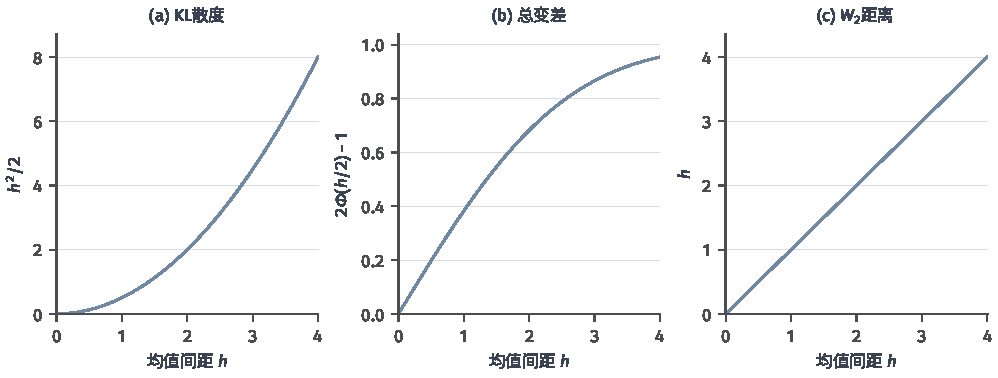
\includegraphics[width=\linewidth]{figures/00-shared/mathematical-preliminaries-lower/01-random-variables-distributions-and-causality/matplotlib/information-gaussian-distances/figure.pdf}
  \caption{同方差高斯位置族的解析式比较。固定\(P=\mathcal N(0,1)\)、\(Q=\mathcal N(h,1)\)，三图分别为\(D_{\mathrm{KL}}=h^2/2\)、\(d_{\mathrm{TV}}=2\Phi(h/2)-1\)与\(W_2=h\)，图中\(h\geq0\)。纵轴分别表达对数代价、事件概率差与搬运位移。}
  \label{fig:information-gaussian-distances}
\end{figure*}

对点质量\(\delta_0,\delta_\varepsilon\)，只要\(\varepsilon\neq0\)，
TV恒为一、两个方向KL均无限，而\(W_r=|\varepsilon|\to0\)。
这是支持移动在不同尺度下的极限差别。
对时间边缘分布\((P_t)\)也可比较这些距离，但它们不决定轨迹机制：
每时刻都为同一公平二元分布，既可能来自反复独立抽样，也可能来自把初次抽样永远复制。
两过程边缘距离为零，时间依赖却完全不同，必须比较联合轨迹。
实际估计MMD或Wasserstein还需考虑核、底层成本、矩和样本量；
高维经验搬运的估计误差可能很大，精确总体公式不自动给出便宜的样本估计。

\section{依赖关系的度量}
\label{sec:information-mutual-relations}

现有差异工具还可以用于两个变量之间的关系。固定它们的真实联合分布，再用各自边缘的独立乘积作参照：两张分布有相同的单变量边缘，差异只来自共同变化。以KL比较这两个对象，便得到互信息，衡量联合规律对独立规律的偏离。

\subsection{基于信息量的依赖度量}
\subsubsection{无条件下的共享信息量}
\label{sec:information-unconditional-mi}

\begin{definition}[互信息]
\label{def:information-mutual-information}
对具有联合分布\(P_{XY}\)的随机元素\(X,Y\)，\term{互信息}
（mutual information, MI）定义为
\begin{equation}
  I(X;Y)=D_{\mathrm{KL}}(P_{XY}\Vert P_X\otimes P_Y).
  \label{eq:information-mutual-information}
\end{equation}
定义适用于一般可测空间，允许值为\(+\infty\)，不要求先存在密度或有限熵。
\end{definition}

Gibbs不等式给出非负性，而且\(I(X;Y)=0\)当且仅当\(X,Y\)独立。
这强于零协方差：例如\(X\)在\(\{-1,0,1\}\)上均匀，\(Y=X^2\)，
协方差为零，但\(Y\)完全由\(X\)确定，互信息为
\(H(Y)=H_{\mathrm b}(1/3)>0\)。
对可数离散变量，定义展开为
\(\sum_{x,y}p(x,y)\log[p(x,y)/(p(x)p(y))]\)；
当\(H(X,Y)<\infty\)时，展开对数并用熵链式法则可得
\begin{equation}
  I(X;Y)=H(X)-H(X\mid Y)=H(Y)-H(Y\mid X).
  \label{eq:information-mi-entropy-reduction}
\end{equation}
所以互信息是观测平均消除的不确定性。连续变量在相关微分熵均有限时也可作相应分解，
但KL定义更一般。例如连续的\(Y=X\)可能使联合分布落在对角线上，
相对于边缘乘积奇异，此时互信息无限，不能强行用有限密度公式计算。

回到例~\ref{ex:information-binary-channel}，有
\(I(X;Y)=\log2-H_{\mathrm b}(\varepsilon)\)。
图~\ref{fig:information-binary-channel-information}中两条曲线相加始终为\(\log2\)；
翻转噪声改变的是观测可提供的信息，而不是公平输入自身的熵。
\begin{figure}[htbp]
  \centering
  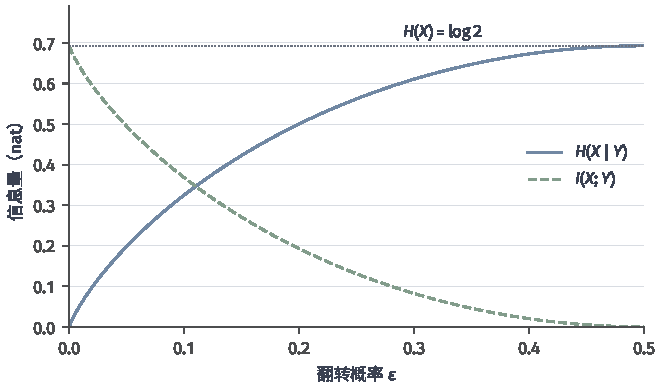
\includegraphics[width=\linewidth]{figures/00-shared/mathematical-preliminaries-lower/01-random-variables-distributions-and-causality/matplotlib/information-binary-channel-information/figure.pdf}
  \caption{公平二元输入通过独立翻转通道后的信息分配（解析式教学图）。蓝实线为剩余条件熵\(H_{\mathrm b}(\varepsilon)\)，绿虚线为互信息\(\log2-H_{\mathrm b}(\varepsilon)\)，均以nat计。输入熵保持不变，零噪声与公平翻转分别对应完整信息与零信息。}
  \label{fig:information-binary-channel-information}
\end{figure}
由于对两个变量分别施加可逆变换会同时推送联合分布与边缘乘积，
互信息继承KL的不变性。这与微分熵随坐标单位改变形成区别。

\subsubsection{条件观测下的剩余依赖}
\label{sec:information-conditional-mi}

已经知道\(Z\)时，应在同一个条件值下判断\(X,Y\)是否还有关系，
再按\(Z\)的发生概率平均。不能把三者的边缘依赖随意相减。

\begin{definition}[条件互信息]
\label{def:information-conditional-mi}
设\(X,Y,Z\)取值于标准Borel空间，因而存在所需正则条件分布。
\term{条件互信息}（conditional mutual information）定义为
\begin{equation}
  I(X;Y\mid Z)
  =\int D_{\mathrm{KL}}\bigl(
    P_{XY\mid z}\Vert P_{X\mid z}\otimes P_{Y\mid z}\bigr)\,P_Z(\mathrm dz).
  \label{eq:information-conditional-mutual-information}
\end{equation}
条件核的版本只需在\(P_Z\)-几乎处处确定；被积量非负，允许结果为\(+\infty\)。
\end{definition}

在不保证正则条件分布存在的一般空间上，不能不加条件地沿用这个条件核定义。
在上述条件下，零条件互信息等价于条件联合核几乎处处等于条件边缘乘积，
也就是前章的条件独立。有限熵时可写成
\(H(X\mid Z)-H(X\mid Y,Z)\)，但非负KL积分是避免无穷相减的基本口径。

条件化并不一定使互信息变小。取独立公平二元变量\(X,Y\)，令\(Z=X\oplus Y\)。
边缘上互信息为零；固定\(Z\)后，\(X\)完全决定\(Y\)，条件互信息为\(\log2\)。
反过来，若\(X=Y=Z\)为同一个公平二元变量，无条件互信息为\(\log2\)，
条件互信息却为零。前者揭示约束，后者去掉已经知道的共享信息。

\subsubsection{信息的链式分解与后处理}
后处理和序贯观测都要用到KL的条件分解。设联合规律满足\(P_{AB}\ll Q_{AB}\)，并存在所需正则条件核。
这推出\(P_A\ll Q_A\)，以及在\(P_A\)-几乎处处的条件值上
\(P_{B\mid A}\ll Q_{B\mid A}\)。联合密度比分解为边缘比与条件比的乘积，
取对数并用塔式性质得到
\begin{equation}
  D_{\mathrm{KL}}(P_{AB}\Vert Q_{AB})
  =D_{\mathrm{KL}}(P_A\Vert Q_A)
   +\mathbb E_{A\sim P_A}
       D_{\mathrm{KL}}(P_{B\mid A}\Vert Q_{B\mid A}).
  \label{eq:information-kl-conditional-chain}
\end{equation}
每个对数比的负部可积，故有限项相加的分解也能按非负扩展值成立；
若绝对连续性失败，对应的条件或边缘项为无限。
把\(Q_{XYZ}\)选为\(P_X\otimes P_{YZ}\)，再按\((X,Y)\)与\(Z\)分组，
第一项是\(I(X;Y)\)，条件项是
\(\mathbb E_{X,Y}D_{\mathrm{KL}}(P_{Z\mid X,Y}\Vert P_{Z\mid Y})
=I(X;Z\mid Y)\)。因此
\[
  I(X;Y,Z)=I(X;Y)+I(X;Z\mid Y).
\]
这证明了互信息链式法则，而不仅是引用熵差记号。

若先观察\(Y\)，再只依据\(Y\)生成摘要\(Z\)，摘要没有另行接触关于\(X\)的资料。因而要检查：压缩或随机处理能否增加它对\(X\)的信息？条件独立\(X\perp Z\mid Y\)精确表达没有额外来源的限制，链式法则则将它转为信息量不增加的结论。
\begin{theorem}[数据处理不等式]
\label{thm:information-data-processing}
若标准Borel随机元素满足Markov关系\(X\to Y\to Z\)，
即\(X\perp Z\mid Y\)，则\(I(X;Z)\leq I(X;Y)\)，允许扩展值。
\end{theorem}
\begin{proof}
用两种顺序分解同一联合信息量：
\[
\begin{aligned}
  I(X;Y,Z)&=I(X;Y)+I(X;Z\mid Y)=I(X;Y),\\
  I(X;Y,Z)&=I(X;Z)+I(X;Y\mid Z)\geq I(X;Z).
\end{aligned}
\]
第一行的条件项由条件独立为零，第二行的条件项非负，合并即得。
证明只作非负项的相加和比较，不需要有限熵，也没有无穷相减。
\end{proof}

处理可以是\(Z=g(Y)\)，也可以是仅依赖\(Y\)的随机通道。
若额外随机性还与\(X\)关联，Markov前提可能不成立。
信息不增加并不保证每个任务的误差严格增加；当丢弃的内容与任务无关时可以取等号。

\subsection{基于距离的依赖度量}
\label{sec:information-distance-dependence}

前章的相关系数只比较中心化乘积的平均，\(Y=X^2\)的对称例子已经说明零相关可以漏掉确定关系。要保留更一般的依赖，可以比较联合特征函数与边缘特征函数的乘积；独立性恰好要求这两个函数在每个频率都相等。频率上的差异还可以转换为样本之间的距离计算。

\subsubsection{距离协方差与距离相关系数}
设\(X\in\mathbb R^p,Y\in\mathbb R^q\)，且\(\mathbb E\|X\|+\mathbb E\|Y\|<\infty\)。记联合及边缘特征函数为\(\varphi_{XY},\varphi_X,\varphi_Y\)，令\(c_d=\pi^{(d+1)/2}/\Gamma((d+1)/2)\)。\term{距离协方差}（distance covariance, dCov）的平方定义为
\begin{equation}
 \mathcal V^2(X,Y)
 =\frac1{c_pc_q}\int_{\mathbb R^{p+q}}
 \frac{|\varphi_{XY}(t,s)-\varphi_X(t)\varphi_Y(s)|^2}
 {\|t\|^{p+1}\|s\|^{q+1}}\,\mathrm dt\,\mathrm ds.
 \label{eq:information-distance-covariance}
\end{equation}
坐标轴是Lebesgue零集，可任意指定被积函数在轴上的值。一阶矩条件使该非负积分有限。再令
\[
 \mathcal R^2(X,Y)=
 \begin{cases}
 \displaystyle\frac{\mathcal V^2(X,Y)}
 {\sqrt{\mathcal V^2(X,X)\mathcal V^2(Y,Y)}},&
 \mathcal V^2(X,X)\mathcal V^2(Y,Y)>0,\\
 0,&\text{否则},
 \end{cases}
\]
其非负平方根称为\term{距离相关系数}（distance correlation, dCor）。它在上述欧氏空间与矩条件下取值于\([0,1]\)，零值当且仅当独立；有限性与归一化界可见原始论证\scite{math-szekely2007dependence}。

零值的识别机制可以直接从积分看出。权重在两条坐标轴外严格为正，零积分意味着两种特征函数几乎处处相等；连续性再把等式扩展到所有频率。特征函数唯一性给出\(P_{XY}=P_X\otimes P_Y\)。反向由独立性立即成立。与互信息不同，这里的有限数值不依赖联合分布相对于边缘乘积具有密度，但它依赖欧氏距离与所规定的矩条件。

\subsubsection{基于成对距离的样本计算}
对观测对\((x_i,y_i)_{i=1}^n\)，先计算距离矩阵\(a_{ij}=\|x_i-x_j\|\)、\(b_{ij}=\|y_i-y_j\|\)，再分别去掉行均值与列均值，加回总体均值：
\[
 A_{ij}=a_{ij}-\bar a_{i\cdot}-\bar a_{\cdot j}+\bar a_{\cdot\cdot},
 \qquad
 B_{ij}=b_{ij}-\bar b_{i\cdot}-\bar b_{\cdot j}+\bar b_{\cdot\cdot}.
\]
这里\(\bar a_{i\cdot}=n^{-1}\sum_j a_{ij}\)、\(\bar a_{\cdot\cdot}=n^{-2}\sum_{ij}a_{ij}\)，其余同理。常用的非负经验量为
\[
 \mathcal V_n^2=\frac1{n^2}\sum_{i,j}A_{ij}B_{ij}.
\]
双中心化去掉仅由单侧位置决定的平均距离，余下的同步变化对应联合依赖；这与直接对原始数值求协方差的观察口径不同。距离公式及其与特征函数积分的等价，按同一原始文献使用，不把含可能无限项的期望差擅自相减。

对上面的三点总体\((X,Y)=(-1,1),(0,0),(1,1)\)，每点概率为\(1/3\)。用三个支持点及其等权重作同样的双中心化，得到总体\(\mathcal V^2(X,Y)=8/81\)、\(\mathcal V^2(X,X)=40/81\)、\(\mathcal V^2(Y,Y)=16/81\)，故\(\mathcal R^2=1/\sqrt{10}>0\)。它识别了协方差为零的关系。实际从未知总体抽取有限样本时，\(\mathcal V_n\)只是随机统计量；非零样本值不是总体依赖的证明，显著性与置换校准由第~\ref{sec:statistics-testing-errors}节处理。

\subsection{基于核嵌入的依赖度量}
\label{sec:information-kernel-dependence}

依赖也可以直接写成两张分布的差：比较真实联合规律\(P_{XY}\)与打散配对后的\(P_X\otimes P_Y\)。前面的MMD已能比较分布；现在选取联合空间上的乘积核
\[
 K((x,y),(x',y'))=k(x,x')\ell(y,y'),
\]
其中\(k,\ell\)是可测有界正定核。\term{Hilbert--Schmidt独立性准则}（Hilbert--Schmidt independence criterion, HSIC）定义为
\begin{equation}
 \operatorname{HSIC}_{k,\ell}(X,Y)
 =\operatorname{MMD}_{K}^{2}(P_{XY},P_X\otimes P_Y).
 \label{eq:information-hsic}
\end{equation}
它量化两种配对规律在乘积特征上的平均差异。若\(K\)在所考察的联合分布类上具有特征性，零HSIC就等价于独立；这是一组足够条件，不能仅由核正定推出。有限维欧氏空间上的高斯乘积核满足所需的识别条件\scite{math-gretton2015hsic}。

展开核均值范数，可以把计算写成有限矩阵运算。令\(K_{ij}=k(x_i,x_j)\)、\(L_{ij}=\ell(y_i,y_j)\)，中心化矩阵为\(\bm H=\bm I-\bm1\bm1^\top/n\)，则经验联合分布与经验边缘乘积的平方MMD为
\[
 \widehat{\operatorname{HSIC}}=\frac1{n^2}
 \operatorname{tr}(\bm K\bm H\bm L\bm H).
\]
这是非负但通常有偏的经验版本，不与无偏估计量混用。取标量线性核\(k(x,x')=xx'\)、\(\ell(y,y')=yy'\)且二阶矩有限时，乘积特征只有\(xy\)，总体HSIC退化为\(\operatorname{Cov}(X,Y)^2\)；在前述\(Y=X^2\)例子中仍为零。这个反例说明丰富特征及核的识别条件为何必要。改用高斯核可以识别该依赖，但有限样本的数值与功效仍受带宽和样本规模影响，核的特征性不保证每批样本都容易检出。

\subsection{基于网格划分的依赖度量}
\label{sec:information-grid-dependence}

核与距离保留了取值位置。另一种做法把二维实值观测划入有限网格，只看网格行列是否独立。对每一种网格计算离散互信息，再允许网格随关系形状变化；网格越细，能表达的结构越多，也越容易把有限样本的偶然排列当作关系，因此总体定义与样本搜索要分开。

\subsubsection{总体最大信息系数}
令\(G\)为\(k\times\ell\)的轴对齐有限网格，\(k,\ell\geq2\)，\(X_G,Y_G\)分别记录\(X,Y\)落入的列与行。总体\term{最大信息系数}（maximal information coefficient）的版本记为
\begin{equation}
 \operatorname{MIC}^{\ast}(X,Y)
 =\sup_G\frac{I(X_G;Y_G)}{\log\min\{k,\ell\}}.
 \label{eq:information-population-mic}
\end{equation}
所有信息量使用相同对数底数，归一化比值因而不受bit或nat的选择影响。这一定义及其与有限样本统计量的关系见Reshef等\scite{math-reshef2016dependence}。分母按网格两侧较小的可用信息量归一化，而不是用样本相关系数归一化。

由于\(I(X_G;Y_G)\leq\min\{H(X_G),H(Y_G)\}\leq\log\min\{k,\ell\}\)，有\(0\leq\operatorname{MIC}^{\ast}\leq1\)。独立时任何网格都独立，故值为零；若总体不独立，存在两个阈值使相应二维累积分布不等于边缘累积概率的乘积，这个\(2\times2\)网格有正互信息，所以总体量严格为正。取公平二元变量\(Y=X\)，网格区分\(0,1\)后互信息为\(\log2\)，得到\(\operatorname{MIC}^{\ast}=1\)。

\subsubsection{样本网格搜索与复杂度限制}
给定\(n\)个观测对，对网格内的经验频率计算互信息，并约束网格规模，得到样本版本
\[
 \operatorname{MIC}_{B,n}
 =\sup_{G:\,k\ell\leq B(n)}
 \frac{\widehat I_G}{\log\min\{k,\ell\}}.
\]
其中\(B(n)\)是预先规定的搜索预算。它与不受样本数限制的总体\(\operatorname{MIC}^{\ast}\)不同；实际算法对网格的近似搜索又不同于该精确上确界。只对一个固定网格证明频率收敛，也不足以证明越来越多网格上的最大值收敛，需要对整个搜索类作统一控制。

若不限制复杂度，偶然排列就能给出极高数值。例如偶数\(n\)个连续样本的横、纵坐标均不并列时，可以用\(n\)列把每个横坐标单独分开，用两行把纵坐标各分一半；每列完全决定所属行，经验互信息为\(\log2\)，归一化值便为\(1\)，即使总体独立也如此。这个\(2n\)格构造说明预算约束的作用。总体依赖量、有限样本估计、独立性检验及关系强度排序各有不同目标，不能把一个较大的MIC值直接解释成显著关系或因果效应。

\section{概率分布的压缩与还原}
\label{sec:information-compression-reconstruction}

无失真编码要求接收者恢复每个符号，连续数值的记录却已经包含近似。以温度记录为例，把\(20.03\)度与\(20.04\)度存成同一个\(20.0\)度，可以节省描述，却改变了还原误差。现在固定源分布\(P_X\)，同时规定存储量与还原代价，研究能够保留多少关于原结果的信息。

\subsection{基于量化的近似还原}
\label{sec:information-quantization}

编码器先把取值区域划成可数个单元\(C_j\)，记录单元索引\(J=q(X)\)；解码器收到\(j\)后输出重构值\(c_j\)，于是\(\widehat X=c_{q(X)}\)。这类以有限或可数代表值近似原结果的操作称为\term{量化}（quantization）。给索引再使用前缀码，只能完整还原\(J\)，不能恢复已在单元内合并的差别。码长和失真分别由\(P(J=j)\)及\(X\)在各单元内的变化决定。

\subsubsection{均匀标量量化与误差尺度}
对步长\(\Delta>0\)，无限范围的最近邻量化器为
\[
 Q_\Delta(x)=\Delta\left\lfloor\frac{x}{\Delta}+\frac12\right\rfloor.
\]
除格点边界的并列约定外，误差\(E=Q_\Delta(X)-X\)满足\(|E|\leq\Delta/2\)，所以\(\mathbb E E^2\leq\Delta^2/4\)。若设备只保留有限个重构值，范围外还会发生饱和；上述界只控制范围内的舍入误差，不能遗漏过载部分。

常见的\(\Delta^2/12\)来自更强的近似：密度在一个单元内变化很小，且过载概率可以忽略时，给定单元的读数近似均匀。对\([-\Delta/2,\Delta/2]\)上的均匀误差直接积分，得到
\[
 \mathbb E E\approx0,\qquad
 \mathbb E E^2\approx\frac1\Delta
 \int_{-\Delta/2}^{\Delta/2}e^2\,\mathrm de
 =\frac{\Delta^2}{12}.
\]
它是高分辨率模型，不是任意输入下的精确方差。若\(X\)总在重构格点上，误差恒为零；若总落在单元同一侧，误差均值也可以不为零。确定性量化误差由\(X\)决定，不能再假定它与\(X\)独立。

以\([0,1]\)均匀源为例，分成\(m\)个等宽单元并用中点还原时，\(\Delta=1/m\)，均方误差精确为\(1/(12m^2)\)，索引熵为\(\log m\)。若\(m=2^b\)，固定长度记录每个索引用\(b\) bit，误差为\(2^{-2b}/12\)；增加一位使误差缩为四分之一。这个精确例子依赖均匀源、等宽单元与中点还原，不能直接搬给非均匀源。

\paragraph{随机扰动与加性噪声模型}
在无饱和的均匀格点量化中，可以加入接收双方共享的独立扰动\(U\sim\operatorname{Unif}[-\Delta/2,\Delta/2)\)，并令\(\widehat X=Q_\Delta(X+U)-U\)。固定\(X=x\)时，\(x+U\)对格宽取余均匀，故还原误差在长度\(\Delta\)的居中区间内均匀，条件分布不依赖\(x\)。这里的零均值、方差\(\Delta^2/12\)与误差独立性来自共享随机扰动及减去它的操作；它们不自动适用于未扰动的量化器。学习时把量化替换为独立均匀噪声，也只是另行选择的训练近似，不是确定性舍入的恒等改写。

\subsubsection{非均匀与向量量化的重构选择}
对\(X\in\mathbb R^d\)与平方误差，量化目标为
\[
 D(q,c)=\mathbb E\|X-c_{q(X)}\|_2^2.
\]
固定单元且二阶矩有限时，条件平方误差分解给出\(c_j=\mathbb E[X\mid X\in C_j]\)，只需对正概率单元计算；固定重构值时，逐点选择最近的\(c_j\)最优。这两条必要的交替最优条件称为Lloyd条件：单元随代表值重新划分，代表值再移到单元的条件均值。每次精确更新不增加失真，但目标不凸，停止点未必是全局最优。\term{向量量化}（vector quantization）联合处理多个坐标，能够利用它们的共同分布，代价是码本存储、搜索与估计更复杂。

若同时考虑索引的熵，最优分配还会改变。给第\(j\)个索引预定理想码长\(r_j=-\log_2p_j\)，比较每个输入的\(\|x-c_j\|^2+\lambda r_j\)，长码索引就需要更大的失真收益才能被选中。更新单元后\(p_j\)也会变化，因此固定概率的最近邻条件与熵约束量化不是同一个优化问题。实际码长另有整数及模型传输代价，不能只报理想熵。

\subsection{失真约束下的最低信息率}
\label{sec:information-rate-distortion}

量化器选定了一种编码与还原规则。为了判断任何规则最低需要多少信息，先放宽到所有条件重构规律\(P_{\widehat X\mid X}\)。固定非负可测失真\(d(x,\widehat x)\)，平均失真按\(P_XP_{\widehat X\mid X}\)计算；互信息则衡量重构结果保留了多少源信息。

\subsubsection{率失真函数与编码含义}
\begin{definition}[率失真函数]
\label{def:information-rate-distortion}
给定源分布\(P_X\)、重构空间和失真\(d\)，定义
\begin{equation}
 R(D)=\inf_{P_{\widehat X\mid X}:\,\mathbb E d(X,\widehat X)\leq D}
 I(X;\widehat X),\qquad D\geq0.
 \label{eq:information-rate-distortion}
\end{equation}
空可行集的下确界约定为\(+\infty\)。使用自然对数时，\(R(D)\)的单位为nat每源符号；比特率为\(R(D)/\log2\)。没有紧性等存在条件时，不把下确界直接写成最小值。
\end{definition}

允许更大失真会扩大可行集合，所以\(R(D)\)不增。对两个重构通道随机选择其中一个，选择概率独立于源；条件互信息与数据处理表明混合通道的信息不超过两者的加权平均，失真则恰为加权平均。这给出\(R(D)\)的凸性，说明随机切换编码方案可以获得中间工作点。

对于独立同分布的有限字母源及有限失真表，率失真编码定理说明：足够长的块编码可以使平均每符号失真接近\(D\)，并以任意高于\(R(D)/\log2\)的比特率实现；低于该值的渐近编码率不能达到同一失真目标\scite{math-cover2006information}。它是长块与平均失真的极限结论，不承诺某个有限块量化器立即达到此界。对连续源还需相应的可测性、可积性与可逼近条件。确定性\(\widehat X=q(X)\)且索引熵有限时，\(I(X;\widehat X)=H(\widehat X)\)，所以前面的量化及熵编码是在这条极限之上的一种可操作方案。

\subsubsection{高斯源平方误差下的率失真界}
设\(X\sim\mathcal N(\mu,\sigma^2)\)，\(\sigma^2>0\)，失真为\((X-\widehat X)^2\)。此时
\begin{equation}
 R(D)=
 \begin{cases}
 \tfrac12\log(\sigma^2/D),&0<D<\sigma^2,\\
 0,&D\geq\sigma^2,\\
 +\infty,&D=0.
 \end{cases}
 \label{eq:information-gaussian-rate-distortion}
\end{equation}
下界可以直接用KL非负性证明，避免先假定所有条件微分熵有限。给定任一失真不超过\(D\)的联合规律，取参考核\(q_D(x\mid\widehat x)\)为均值\(\widehat x\)、方差\(D\)的高斯密度。真实源密度\(p_X\)严格为正，且\(\log(q_D(X\mid\widehat X)/p_X(X))\)由二阶矩条件可积。相对熵的密度比分解给出
\[
\begin{aligned}
 I(X;\widehat X)
 &=D_{\mathrm{KL}}(P_{X\widehat X}\Vert q_D\,P_{\widehat X})
   +\mathbb E\log\frac{q_D(X\mid\widehat X)}{p_X(X)}\\
 &\geq\frac12\log(\sigma^2/D)+\frac12
       -\frac{\mathbb E(X-\widehat X)^2}{2D}
 \geq\frac12\log(\sigma^2/D).
\end{aligned}
\]
若联合规律相对于上述参考不绝对连续，第一项与互信息均为无穷，仍满足下界；没有作无穷相减。参考核把“还原误差不超过\(D\)”转成一项可计算的平均对数密度，KL非负性补上剩余的非负部分。

对\(0<D<\sigma^2\)，取独立的\(\widehat X\sim\mathcal N(\mu,\sigma^2-D)\)、\(N\sim\mathcal N(0,D)\)，再令\(X=\widehat X+N\)。这先构造联合分布，再取其正则条件分布作为重构通道；它具有所需的源边缘、失真\(D\)和恰好取等号的互信息，故达到下界。\(D\geq\sigma^2\)时恒定重构\(\widehat X=\mu\)已可行且信息为零。\(D=0\)要求连续源被精确还原，联合分布与边缘乘积奇异，互信息无限。这里的最优联合高斯通道不是普通逐符号标量量化器，二者的实现约束不同。

\subsection{预算约束下的码率分配}
\label{sec:information-rate-allocation}

\subsubsection{独立高斯分量的反注水分配}
若正交变换后有独立高斯分量\(X_j\sim\mathcal N(0,\lambda_j)\)，\(\lambda_j>0\)，总平方失真为各坐标误差之和。对每个分量选失真\(D_j\leq\lambda_j\)，总率为\(\tfrac12\sum_j\log(\lambda_j/D_j)\)，总失真为\(\sum_jD_j\)。这确实给出向量高斯的最优值：联合源熵可加，条件熵不超过各坐标误差熵之和，得到相同下界；独立使用上一小节的反向高斯通道则同时取到等号。

在\(0<D<\sum_j\lambda_j\)下，最小化总率并限制总失真不超过\(D\)，Lagrange一阶条件在未触边分量给出\(-1/(2D_j)+\beta=0\)。于是
\[
 D_j=\min\{\lambda_j,\theta\},\qquad
 \sum_j\min\{\lambda_j,\theta\}=D,
 \qquad
 R(D)=\frac12\sum_j\max\{0,\log(\lambda_j/\theta)\}.
\]
所有需编码方向分配相同的剩余误差\(\theta\)，方差低于阈值的方向直接以均值还原、不再分配比特；这称为反注水（reverse water-filling）。例如\((\lambda_1,\lambda_2)=(4,1)\)、\(D=2\)时，\(\theta=1\)，两方向失真均为\(1\)，第一方向分配\(1\) bit，第二方向为零。分配依据是高斯独立分量的方差；仅仅进行某个固定变换，不足以保证一般数据也满足这一模型。

\subsubsection{有限编码方案的码率与失真权衡}
实际编码器常只允许有限组工作点\((R_j,D_j)\)。给定\(\beta>0\)，最小化\(R_j+\beta D_j\)把存储与还原代价换成同一目标；若采用\(D_j+\lambda R_j\)，则\(\lambda=1/\beta\)。在光滑凸的率失真边界上，切线条件为\(R'(D)=-\beta\)，权重因此对应边界斜率，而不是任意经验常数的理论保证。

有限候选不一定能用某个权重取得所有预算最优点。例如\((R,D)=(0,4),(1,3),(2,0)\)中，预算\(R\leq1\)下第二点优于第一点；但要使其\(R+\beta D\)同时不大于两端，须有\(\beta\geq1\)及\(\beta\leq1/3\)，不可能成立。允许按比例切换两端方案才得到下凸包上的中间点；不允许切换时，约束优化与加权优化有不同的可达范围。逐块决策若还共享总码率、参考重构或上下文概率，块间也不能在未处理这些耦合时直接独立最小化。

\section{概率分布的收敛}
\label{sec:information-distribution-convergence}

分布近似通常形成一列规律\(P_1,P_2,\ldots\)。如果小位移被逐步消除，希望连续读数的平均也随之稳定；但少量概率同时移向远处时，无界读数仍可能改变。我们先用有界连续函数规定弱收敛，再检查能否保住总概率，以及何种额外尾部条件允许更强的距离收敛。这里比较的是分布，暂不要求把不同索引的随机变量放在同一基础空间上；共同空间上的随机结果收敛由\BookChapterRef{chap:random-sequences-and-processes}{第~\ref{chap:random-sequences-and-processes}章}讨论。

\subsection{基于连续探针的弱收敛}
\label{sec:information-continuous-probe-convergence}
\begin{definition}[概率测度的弱收敛]
\label{def:information-weak-measure-convergence}
对同一度量空间上的Borel概率测度\(P_n,P\)，若对每个有界连续实函数\(h\)均有
\(\int h\,\mathrm dP_n\to\int h\,\mathrm dP\)，就称\(P_n\)弱收敛到\(P\)，记作\(P_n\Rightarrow P\)。这种\term{概率测度的弱收敛}（weak convergence of probability measures）只比较各测度的积分，不要求随机变量在同一基础空间上逐点接近。
\end{definition}
有界连续函数是比较分布的探针：连续性不放大微小位置移动，有界性不让极少量远处质量主导结果。实数上的这个定义等价于在\(F\)的全部连续点上有\(F_n(x)\to F(x)\)，也就与随机变量的依分布收敛一致。例如\(\delta_{1/n}\Rightarrow\delta_0\)，但对集合\(\{0\}\)，前者始终赋概率零、后者赋概率一；弱收敛不要求每个事件的概率都收敛。

\begin{theorem}[Portmanteau的常用形式]
\label{thm:rv-portmanteau}
在Polish空间\(E\)上，Borel概率测度\(P_n\Rightarrow P\)等价于下列任一条件：
对每个闭集\(C\)，\(\limsup_nP_n(C)\leq P(C)\)；
对每个开集\(G\)，\(\liminf_nP_n(G)\geq P(G)\)；
对每个满足\(P(\partial A)=0\)的Borel集\(A\)，\(P_n(A)\to P(A)\)。
弱收敛还给出每个非负下半连续函数\(c\)的积分下界
\[
\int c\,\mathrm dP\leq\liminf_n\int c\,\mathrm dP_n.
\]
\end{theorem}
这里Polish指拓扑可由完备可分度量诱导。闭集条件可由连续函数
\(h_k(x)=\max\{1-k\,d(x,C),0\}\)从上逼近\(\mathbb I_C\)得到，开集条件再取补集。若边界质量为零，对内部和闭包夹逼即得事件概率收敛。非负下半连续函数可由递增的有界连续函数逼近，先对每个逼近函数取弱极限，再用单调收敛，得到积分不等式。这也解释了为何非负成本的极限只能先得到下界；无界一般函数需要额外的尾部控制。

\subsection{紧性与弱收敛子列}
\label{sec:rv-weak-convergence}

上面的定义检验一列分布是否接近指定的极限。现在还没有候选极限，要先问这列分布是否至少能抽出弱收敛子列。路径分布与最优传输的联合分布也会遇到这个存在性问题，不能仅凭每张分布各自归一化就断定极限仍保有总概率。

弱收敛的另一困难是质量可能不断远移，使任何候选极限都留不住总概率。需要紧性把绝大部分质量统一留在可控区域。
\begin{definition}[紧概率测度与一致紧族]
\label{def:information-tightness}
度量空间上的Borel概率测度\(P\)称为\term{紧的}，若对每个
\(\varepsilon>0\)存在紧集\(K\)，使\(P(K^{\mathsf c})<\varepsilon\)。
一族概率测度\(\mathcal P\)称为\term{一致紧的}，若对每个\(\varepsilon>0\)可取同一个紧集，使
\(\sup_{Q\in\mathcal P}Q(K^{\mathsf c})<\varepsilon\)。
\end{definition}
\begin{theorem}[Prokhorov定理]
\label{thm:rv-prokhorov}
Polish空间上的Borel概率测度族一致紧，当且仅当它相对弱序列紧，即每个序列都能抽出弱收敛到该空间上某个概率测度的子列。每个单独的Borel概率测度都是紧的。
\end{theorem}
定理保证可抽取子列，不保证所有子列具有同一极限；还需识别极限才能证明整列收敛。单个测度紧也不等于一个族一致紧。

一致紧的失败通常来自质量的“逃逸”：每个成员各自都紧，取共同紧集时却留不住质量。
以\(P_n=\delta_n\)为例，每个\(P_n\)都紧，但任意固定\(R\)下
\(P_n([-R,R])=0\)对所有\(n>R\)成立，任何共同紧集外的质量都是\(1\)。
这个族因此不一致紧，也抽不出弱收敛子列——质量在不断往新的位置移动。
与之对照，取\(P_n=\mathcal N(0,1/n)\)，虽然\(n\)越大分布越集中，
但它们都集中在\(0\)附近：由Chebyshev不等式，
\(P_n(|x|>R)\leq1/(nR^2)\leq1/R^2\)对所有\(n\)成立，
取足够大的\(R\)即可同时控制每一条，所以一致紧，并弱收敛到\(\delta_0\)。
两种情形里取值范围的直观都在变化，区分在于质量能否被同一个区域同时留住，
而不是支持集有多大：紧性约束的正是这种“同时留住”的能力。

在\(\mathbb R^d\)中，若\(\sup_n\mathbb E\|X_n\|^p\leq C<\infty\)，其中\(p>0\)，则
\[
\sup_n\mathbb P(\|X_n\|>R)\leq C/R^p.
\]
闭球紧，故这些分布一致紧。在一般无限维空间，闭有界集未必紧，单有范数矩界不能照搬此论证。后面路径收敛还需控制短时间内的振荡；
第~\ref{sec:information-optimal-coupling-existence}节
则在固定边缘下构造共同紧集。二者都使用本节的通用定义，不是固定测度下的积分交换。

\subsection{基于特征函数的收敛判定}
\label{sec:information-characteristic-convergence}

独立累计量的特征函数可以相乘，往往比直接计算分布函数容易。但即使各个特征函数逐点有极限，也还要保证这个极限对应一张概率分布。下面在原点的连续性条件完成这项检查，并把函数极限转回依分布收敛。
\begin{theorem}[L\'evy连续性定理]
  \label{thm:probability-levy-continuity}
  令\(X_n\)的特征函数为
  \(\varphi_n(t)=\mathbb{E}[e^{\mathrm{i}tX_n}]\)。
  若\(\varphi_n(t)\)对每个\(t\in\mathbb{R}\)收敛到函数\(\varphi(t)\)，且
  \(\varphi\)在\(t=0\)处连续，则\(\varphi\)是某个概率分布的特征函数；若
  \(X\)服从该分布，则\(X_n\Rightarrow X\)。反过来，若\(X_n\Rightarrow X\)，则
  \(\varphi_n(t)\to\varphi_X(t)\)对每个\(t\)成立。
\end{theorem}

Prokhorov定理与L\'evy连续性定理的完整证明按上述Polish空间及实值特征函数条件使用，可见Kallenberg\scite{math-kallenberg2021probability}。这里给出定理的使用条件与排除的失败情形，不把它们当作任意函数极限的存在性结论。该连续性定理给出从特征函数逐点极限到依分布收敛的接口。“极限在零点连续”不能省略；它排除
极限质量逃向无穷远而不再对应概率分布的情形。


\subsection{分布距离收敛与尾部条件}
\label{sec:information-metric-convergence}

前面的分布距离会给出不同强度的收敛。\(d_{\mathrm{TV}}(P_n,P)\to0\)统一控制所有事件，也就控制每个有界连续函数的期望，因而推出弱收敛；\(D_{\mathrm{KL}}(P_n\Vert P)\to0\)再由Pinsker推出TV收敛。逆向都需要额外条件：\(\delta_{1/n}\Rightarrow\delta_0\)，但两分布不重叠，TV始终为一，前向KL无限。

\paragraph{弱收敛与搬运矩的结合}
对Polish度量空间上的\(P_n,P\in\mathcal P_r\)，\(1\leq r<\infty\)，有如下判定：
\begin{equation}
 W_r(P_n,P)\longrightarrow0
 \quad\Longleftrightarrow\quad
 \begin{cases}
 P_n\Rightarrow P,\\
 \displaystyle\int d(x,x_0)^r\,\mathrm dP_n
 \longrightarrow\int d(x,x_0)^r\,\mathrm dP.
 \end{cases}
 \label{eq:information-wasserstein-convergence}
\end{equation}
等价地，弱收敛之外需对\(d(x,x_0)^r\)有统一的尾部可积控制；这一标准结论沿用定义~\ref{def:information-wasserstein-distance}中的矩条件，可见Villani\scite{math-villani2009transport}。必要性可沿近最优耦合使用距离三角不等式和\(L^r\)范数连续性理解；充分性则在共同的大紧集内逼近配对，并用尾部可积性消去紧集外的成本。矩有界只保证紧性，不自动保证尾部积分一致趋零。

例如\(P_n=(1-1/n)\delta_0+(1/n)\delta_n\)弱收敛到\(\delta_0\)，甚至TV为\(1/n\)，但所有质量只能搬往零点，故
\[
 W_r^r(P_n,\delta_0)=\frac1n n^r=n^{r-1}.
\]
\(r=1\)时平均搬运代价恒为一，\(r>1\)时还会增长。越来越少的远处质量可以逃过有界探针，却仍主导无界成本。这也是下一节对无界评价函数另加敏感性或尾部条件的原因。

\paragraph{核均值收敛的识别条件}
若核有界且连续，弱收敛通过核期望展开给出\(\operatorname{MMD}(P_n,P)\to0\)。反向需要核均值差能够控制弱拓扑；仅有“零MMD意味着同分布”的特征性，是单个分布对的识别条件，不在一般空间上自动提供这一序列结论。比较收敛时，应核对核的拓扑条件、底层空间和尾部要求，而不是仅根据距离都为零时的等号条件推断相同的极限强度。

\section{概率分布变化下的期望响应}
\label{sec:information-task-stability}
\label{sec:information-fixed-evaluation}

同一个评价函数在两张分布下有两个期望，我们现在要控制它们的差。若函数取值有界，事件概率差足以给出控制；若函数随位置变化缓慢，可以利用搬运距离；若参考分布能控制函数尾部，则可结合指数矩与KL。以下分别改变已知条件，函数本身和所比较的两张分布仍要明确固定。

\subsection{有界函数的期望响应}
\label{sec:information-bounded-evaluation}

设固定可测损失\(f\)取值于\([0,1]\)。逐点恒等式
\(f(x)=\int_0^1\mathbb I\{f(x)>t\}\,\mathrm dt\)与Tonelli定理给出
\[
  |\mathbb E_Pf-\mathbb E_Qf|
  \leq\int_0^1|P(f>t)-Q(f>t)|\,\mathrm dt
  \leq d_{\mathrm{TV}}(P,Q).
\]
这也说明事件概率控制为何足以控制所有这一范围内的损失。
若\(a<b\)且\(a\leq f\leq b\)，对\((f-a)/(b-a)\)使用同一式子，得到
\[
  |\mathbb E_Pf-\mathbb E_Qf|
  \leq(b-a)d_{\mathrm{TV}}(P,Q).
\]
若\(a=b\)，函数为常量，两侧期望差为零，这个上界仍成立。
特别地，\(|f|\leq1\)时常数是\(2\)，不能把它与\(0\leq f\leq1\)混用。
取两点上的\(P=\delta_0,Q=\delta_1\)和\(f(0)=-1,f(1)=1\)，
期望差为\(2\)，已经表明这个因子不能删除。
在\(a<b\)时结合Pinsker，还可用\((b-a)\sqrt{D_{\mathrm{KL}}(P\Vert Q)/2}\)控制期望差；
若KL无限，这个途径不给出有限信息，但TV界仍有效。

对罕见失败事件，除了TV的加性误差，还可以利用似然比高阶矩。
设\(P\ll Q\)、\(L=\mathrm dP/\mathrm dQ\)，并且某个\(\alpha>1\)满足
\(D_\alpha(P\Vert Q)<\infty\)。由H\"older不等式，
\[
  P(A)=\mathbb E_Q[L\mathbb I_A]
  \leq(\mathbb E_QL^\alpha)^{1/\alpha}
       (\mathbb E_Q\mathbb I_A^{\alpha/(\alpha-1)})^{(\alpha-1)/\alpha}.
\]
代入R\'enyi散度定义，得到
\begin{equation}
  P(A)\leq
  \exp\!\left\{\frac{\alpha-1}{\alpha}D_\alpha(P\Vert Q)\right\}
  Q(A)^{(\alpha-1)/\alpha}.
  \label{eq:information-renyi-event-bound}
\end{equation}
若\(Q(A)=0\)，绝对连续直接给出\(P(A)=0\)，无需计算无穷与零的乘积。
若\(Q(A)=0<P(A)\)，所需方向的绝对连续已经失败，相应散度无限。
例如\(D_2(P\Vert Q)\leq\log4\)、\(Q(A)\leq10^{-4}\)时，
上界为\(2\sqrt{10^{-4}}=0.02\)。这是从参考规律\(Q\)到目标规律\(P\)
的单向风险迁移，不保证反向同样成立。

有界性不能只在常见样本上成立。取
\(Q=\delta_0\)、\(P_\varepsilon=(1-\varepsilon)\delta_0+
\varepsilon\delta_{1/\varepsilon}\)，对无界函数\(f(x)=x\)，
TV为\(\varepsilon\)，期望差却恒为\(1\)。少量尾部质量足以破坏
只依赖TV的小误差结论，必须另外控制函数增长或分布尾部。

\subsection{敏感性约束下的期望响应}
\label{sec:information-sensitive-evaluation}

若损失不会因输入小幅移动而剧变，就应让这种敏感性进入界。
设\(P,Q\in\mathcal P_1(\mathcal X)\)，且
\(|f(x)-f(y)|\leq Ld(x,y)\)。由于
\(|f(x)|\leq|f(x_0)|+Ld(x,x_0)\)，两边期望均有限。
任意耦合\(\gamma\in\Pi(P,Q)\)满足
\[
  |\mathbb E_Pf-\mathbb E_Qf|
  =\left|\int(f(x)-f(y))\,\mathrm d\gamma\right|
  \leq L\int d(x,y)\,\mathrm d\gamma.
\]
对耦合取下确界便得到
\[
  |\mathbb E_Pf-\mathbb E_Qf|\leq LW_1(P,Q).
\]
这也可由式~\eqref{eq:information-kr-duality}直接读出。
界不要求函数有界，但同时使用了一阶矩和相对于所选距离的Lipschitz条件。

对\(\delta_0,\delta_\varepsilon\)，其中\(\varepsilon>0\)，
均值函数\(f(x)=x\)的变化恰为\(\varepsilon=W_1\)，
事件函数\(g(x)=\mathbb I\{x>0\}\)的变化却为\(1\)。
后者在零附近不连续，不属于统一Lipschitz类。
图~\ref{fig:information-small-shift-task}把同一质量位移对应的这两种评价分开显示；
小搬运距离确实保护平滑评价，但不能据此声称所有阈值事件都稳定。
\begin{figure}[htbp]
  \centering
  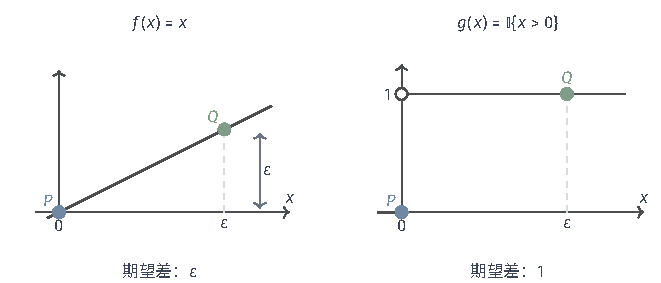
\includegraphics[width=\linewidth]{figures/00-shared/mathematical-preliminaries-lower/01-random-variables-distributions-and-causality/tikz/information-small-shift-task/figure.pdf}
  \caption{同一小位移对两种固定评价的影响。取\(P=\delta_0\)、
  \(Q=\delta_\varepsilon\)、\(\varepsilon>0\)，底层距离为绝对值。
  左图的\(1\)-Lipschitz函数\(f(x)=x\)变化\(\varepsilon\)；
  右图的事件函数\(\mathbb I\{x>0\}\)变化\(1\)。横向位置仅作示意，
  结论对任意正的\(\varepsilon\)成立。}
  \label{fig:information-small-shift-task}
\end{figure}

MMD提供另一种敏感性约束。若同一损失\(f\)属于核\(k\)的RKHS
\(\mathcal H_k\)，且核均值存在，则再生性质和Cauchy--Schwarz不等式给出
\[
  |\mathbb E_Pf-\mathbb E_Qf|
  =|\langle f,\bm\mu_P-\bm\mu_Q\rangle_{\mathcal H_k}|
  \leq\|f\|_{\mathcal H_k}\operatorname{MMD}_k(P,Q).
\]
下标\(k\)显式标明这里沿用的核空间和MMD。
必须知道\(f\)属于该空间及其范数；核具有特征性只保证分离分布，
不自动给出任意任务函数的有限范数。
同样，若底层成本只比较图像亮度，而任务依赖没有计入成本的位置变化，
不能声称损失相对于该成本是Lipschitz。成本与核是任务假设的一部分。

\subsection{指数矩约束下的期望响应}
\label{sec:information-change-measure}

有些评价函数既无统一上界，也没有相对于所选距离的全局Lipschitz常数。例如，以绝对温差\(|x-y|\)为距离、用平方读数\(g(x)=x^2\)评价高温时，\(|g(x+1)-g(x)|=|2x+1|\)没有统一上界，上一节的有限Lipschitz常数因而不可用。若参考分布\(Q\)下\(g\)的矩母函数在零点附近有限，仍可通过指数矩控制尾部，再结合目标分布\(P\)相对\(Q\)的KL来控制期望变化。这里需要核验的是\(\mathbb E_Qe^{\lambda g}\)，不只是温度变量\(X\)自身的矩母函数；例如零均值、方差为\(\sigma^2>0\)的高斯读数满足\(\mathbb E_Qe^{\lambda X^2}=(1-2\lambda\sigma^2)^{-1/2}\)，其有限范围为\(\lambda<1/(2\sigma^2)\)。这个例子只提供有限参数范围的指数矩控制，不满足后文对所有实参数要求的次高斯条件。换测度可以借助密度比把一个分布下的期望改写为另一个分布下的加权期望；下面用KL和指数矩代替密度比的逐点控制。
证明的关键是指数倾斜：按\(e^f\)重新加权参考分布，使较大函数值获得更多质量，再用新分布与目标分布的KL非负性控制期望。

图~\ref{fig:information-square-exponential-moment}固定同一个标准高斯读数，只改变被评价的函数。读数\(X\)的指数矩对所有实参数有限，但平方读数\(X^2\)在\(\lambda\geq1/2\)时已经无限。后面的换测度界因而必须把评价函数和允许的指数参数范围一并列入条件。

\begin{figure}[htbp]
  \centering
  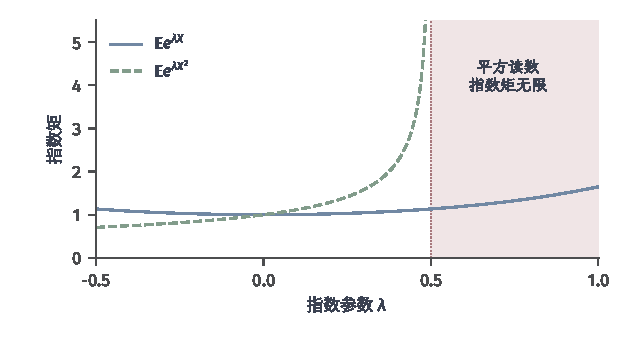
\includegraphics[width=105mm]{figures/00-shared/mathematical-preliminaries-lower/01-random-variables-distributions-and-causality/matplotlib/information-square-exponential-moment/figure.pdf}
  \caption{同一标准高斯变量的两种指数矩。蓝实线为\(\mathbb E e^{\lambda X}=e^{\lambda^2/2}\)，绿虚线为\(\mathbb E e^{\lambda X^2}=(1-2\lambda)^{-1/2}\)，后者只在\(\lambda<1/2\)有限。浅红区域标出平方读数指数矩无限的参数范围；纵轴上方截断了趋于无限的绿线，未将该区域绘成有限数值。}
  \label{fig:information-square-exponential-moment}
\end{figure}

\begin{theorem}[Donsker--Varadhan变分表达]
\label{thm:information-donsker-varadhan}
设\(P\ll Q\)。对每个有界可测实函数\(f\)，
\begin{equation}
  D_{\mathrm{KL}}(P\Vert Q)
  \geq\mathbb E_Pf-\log\mathbb E_Qe^f.
  \label{eq:information-dv-lower}
\end{equation}
而且在扩展实数意义下，
\begin{equation}
  D_{\mathrm{KL}}(P\Vert Q)
  =\sup_{f\ \text{有界可测}}\{\mathbb E_Pf-\log\mathbb E_Qe^f\}.
  \label{eq:information-dv-variational}
\end{equation}
\end{theorem}
\begin{proof}
给定有界\(f\)，令\(Z_f=\mathbb E_Qe^f\)，并定义
\[
  \frac{\mathrm dQ_f}{\mathrm dQ}=\frac{e^f}{Z_f}.
\]
因\(0<Z_f<\infty\)，且密度比严格正，\(Q_f\)与\(Q\)等价。
若\(D_{\mathrm{KL}}(P\Vert Q)<\infty\)，对数密度比可积，
乘法法则给出完整的倾斜恒等式
\[
\begin{aligned}
  D_{\mathrm{KL}}(P\Vert Q_f)
  &=\mathbb E_P\left[\log\frac{\mathrm dP}{\mathrm dQ}-f+\log Z_f\right]\\
  &=D_{\mathrm{KL}}(P\Vert Q)-\mathbb E_Pf+\log Z_f.
\end{aligned}
\]
左侧非负即得下界；若原KL无限，右侧有限，下界仍成立。

为证明上确界恰好等于KL，不能直接假设\(\log(\mathrm dP/\mathrm dQ)\)有界。
记\(L=\mathrm dP/\mathrm dQ\)，在\(L=0\)处令\(\log L=-\infty\)，取
\[
  f_n=\max\{-n,\min\{\log L,n\}\}.
\]
由于\(P(L=0)=0\)，且
\(\mathbb E_P(\log L)^-=\int_{\{L<1\}}-L\log L\,\mathrm dQ<\infty\)，
负部由支配收敛、正部由单调收敛可知
\(\mathbb E_Pf_n\to D_{\mathrm{KL}}(P\Vert Q)\)，允许极限无限。
另一方面，\(e^{f_n}\to L\)，且\(e^{f_n}\leq1+L\)。
在\(Q\)下支配收敛给出\(\mathbb E_Qe^{f_n}\to1\)，
故对应变分值趋向KL。结合已证上界，得到等式。
若\(\log L\)本身有界，它直接取到等号；一般只保证截断序列逼近。
\end{proof}

取两点均匀参考分布\(Q=(1/2,1/2)\)，\(f=(0,\log3)\)，则
\(Z_f=2\)、\(Q_f=(1/4,3/4)\)。此时
\(\mathbb E_{Q_f}f=(3/4)\log3\)，
\(D_{\mathrm{KL}}(Q_f\Vert Q)=(3/4)\log3-\log2\)，
两者之差正是\(\log Z_f\)。
这次倾斜只改变概率权重，没有改变样本的取值。

现在令\(g\)允许无界。假设\(P\ll Q\)、\(g\in L^1(P)\)，并且对所选
\(\lambda>0\)有\(\mathbb E_Qe^{\lambda g}<\infty\)。
取\(g_n=\max\{-n,\min\{g,n\}\}\)，将定理用于\(\lambda g_n\)。
因\(|g_n|\leq|g|\)、\(e^{\lambda g_n}\leq1+e^{\lambda g}\)，
分别在\(P,Q\)下支配收敛，得到
\begin{equation}
  \mathbb E_Pg
  \leq\frac{D_{\mathrm{KL}}(P\Vert Q)+\log\mathbb E_Qe^{\lambda g}}{\lambda}.
  \label{eq:information-change-measure-expectation}
\end{equation}
KL有限才能让这个界提供有限的控制。
若还知道\(g\in L^1(Q)\)，且在\(Q\)下对所有\(t\in\mathbb R\)满足
\[
  \log\mathbb E_Qe^{t(g-\mathbb E_Qg)}\leq t^2\sigma^2/2,
\]
则分别对\(g-\mathbb E_Qg\)和其相反数应用上式，得到
\[
  |\mathbb E_Pg-\mathbb E_Qg|
  \leq\frac{D_{\mathrm{KL}}(P\Vert Q)}{\lambda}+\frac{\lambda\sigma^2}{2}.
\]
当KL与\(\sigma^2\)都严格正且有限时，
取\(\lambda=\sqrt{2D_{\mathrm{KL}}(P\Vert Q)/\sigma^2}\)，得到
\begin{equation}
  |\mathbb E_Pg-\mathbb E_Qg|
  \leq\sqrt{2\sigma^2D_{\mathrm{KL}}(P\Vert Q)}.
  \label{eq:information-subgaussian-change-measure}
\end{equation}
KL为零时\(P=Q\)；\(\sigma^2=0\)时\(g\)在\(Q\)下为常量，
由绝对连续在\(P\)下也如此，所以这两个边界情形仍成立。
对\(Q=\mathcal N(0,1)\)、\(P=\mathcal N(m,1)\)、\(g(x)=x\)，
方差代理为\(1\)，KL为\(m^2/2\)，上界恰等于真实期望差\(|m|\)。
这个界固定了评价函数及两张概率规律。若评价函数又根据同一批记录选出，函数与样本会产生联合依赖；第~\ref{sec:information-data-dependent-evaluation}节将在上述期望响应工具上处理这种选择。

\section{概率分布的优化}
\label{sec:information-variational-learning}

比较分布时，两张规律已经给出；优化分布时，至少一张规律需要选择。收益和矩条件可以决定希望得到的规律；给定目标与候选表示后，可以求最接近目标的分布；固定两个边缘以后，还可以选择成本最小的联合配对。三项任务改变的未知量不同，下面各自建立可行集合和目标，再核对最优解的存在与求解条件。

\subsection{目标约束下的分布选择}
\label{sec:information-target-distribution}

为了得到一张新的概率规律，可以规定平均收益，并限制它偏离参考分布的程度；也可以只给出均值等矩条件，在相容规律中最大化熵。此时待求对象是目标分布本身。约束确定可行范围，收益或熵确定选择方向，指数形式则由这些优化条件推导出来。

\subsubsection{参考分布下的收益与偏离权衡}
\label{sec:information-gibbs-optimization}

设\(P_0\)是可以采样的参考规律，\(f\)为有界可测收益。
若只最大化\(\mathbb E_Qf\)，收益达到最大值且允许在最大值点集中质量时，可以选择这样的点质量；最大值点不唯一时，也可以在整个最大值集合上分配概率，未必得到退化分布。但最高收益不一定达到。以\(P_0\)为\((0,1)\)上的均匀分布、\(f(x)=x\)为例，对整数\(n\geq1\)，密度\(\mathrm dQ_n/\mathrm dP_0=nx^{n-1}\)满足
\[
 \begin{gathered}
 \mathbb E_{Q_n}f=\int_0^1 nx^n\,\mathrm dx=\frac{n}{n+1}\longrightarrow1,\\
 \mathbb E_Qf<1\quad\text{对所有集中在 }(0,1)\text{ 上的概率分布 }Q.
 \end{gathered}
\]
因此这里只有上确界，没有实现收益\(1\)的最优分布；若\(f\)为常量，所有可行分布反而都最优。此外，约束\(Q\ll P_0\)会排除参考分布零质量点上的点质量。引入KL惩罚，是在追求收益的同时限制相对参考规律的概率偏离，而不是预设所有无惩罚问题都有无意义的点质量解。
\begin{theorem}[Gibbs变分式]
\label{thm:information-gibbs-variational}
对有界可测\(f\)，
\begin{equation}
  \log\mathbb E_{P_0}e^f
  =\sup_{Q\ll P_0}\{\mathbb E_Qf-D_{\mathrm{KL}}(Q\Vert P_0)\}.
  \label{eq:information-gibbs-variational}
\end{equation}
KL无限时目标约定为\(-\infty\)，唯一最优分布为
\[
  \frac{\mathrm dQ^\star}{\mathrm dP_0}
  =\frac{e^f}{Z_f},\qquad Z_f=\mathbb E_{P_0}e^f.
\]
\end{theorem}
\begin{proof}
有界性保证\(0<Z_f<\infty\)，且\(Q^\star\)与\(P_0\)等价。
对任何有限KL的\(Q\ll P_0\)，
\[
  \log\frac{\mathrm dQ}{\mathrm dQ^\star}
  =\log\frac{\mathrm dQ}{\mathrm dP_0}-f+\log Z_f.
\]
各项在\(Q\)下可积，故倾斜恒等式给出
\[
  \mathbb E_Qf-D_{\mathrm{KL}}(Q\Vert P_0)
  =\log Z_f-D_{\mathrm{KL}}(Q\Vert Q^\star)\leq\log Z_f.
\]
无限KL候选的目标已为\(-\infty\)。对\(Q^\star\)，
\(\log(\mathrm dQ^\star/\mathrm dP_0)=f-\log Z_f\)有界，
所以自身收益与KL都有限，可以直接代入取到等号。
Gibbs不等式的等号条件说明最优分布唯一。
\end{proof}

这里优化的是分布，Donsker--Varadhan表达优化的则是测试函数；
两条变分式共用同一倾斜恒等式，却交换了固定对象和优化对象。
允许无界\(f\)时，至少需要\(0<Z_f<\infty\)才能定义\(Q^\star\)；
若还满足\(\mathbb E_{P_0}[e^f|f|]<\infty\)，
则\(f\in L^1(Q^\star)\)，最优表达中的两项都有限。
对其他候选，也须限制到\(f\in L^1(Q)\)且KL有限的定义域。

只有归一化常数有限并不够。例如在整数\(k\geq1\)上取
\(P_0(k)=C e^{-k}/k^2\)、\(f(k)=k\)，其中\(C\)归一化\(P_0\)。
则\(Z_f=C\sum_{k\geq1}k^{-2}<\infty\)，而\(Q^\star(k)\)正比于\(k^{-2}\)，
导致\(\mathbb E_{Q^\star}f=\infty\)且KL无限。
此时不能把\(Q^\star\)代入\(\infty-\infty\)。
若\(f\)为有限实值且\(Z_f<\infty\)，令
\(Z_n=\mathbb E_{P_0}[e^f\mathbb I_{\{|f|\leq n\}}]\)，在\(Z_n>0\)时取
\[
  \frac{\mathrm dQ_n}{\mathrm dP_0}
  =\frac{e^f\mathbb I_{\{|f|\leq n\}}}{Z_n}.
\]
其收益和KL有限，目标恰为\(\log Z_n\to\log Z_f\)。
因而在有限目标定义域上仍可逼近上确界，不必有可直接代入的最优分布。

对有界收益\(r\)加入温度\(\beta>0\)，令\(f=r/\beta\)，可得
\[
  \sup_{Q\ll P_0}\{\mathbb E_Qr-\beta D_{\mathrm{KL}}(Q\Vert P_0)\}
  =\beta\log\mathbb E_{P_0}e^{r/\beta},\qquad
  Q^\star\propto P_0e^{r/\beta}.
\]
较小温度更偏向高收益区域，也可能使重要性权重集中、采样方差增大。
KL正则描述相对于\(P_0\)的概率偏离；若某种失败事件必须受控，
仍需用上一节的风险迁移条件或另加约束，不能把正则项本身当成安全保证。

图~\ref{fig:information-gibbs-temperature-weights}用三个结果展示温度的作用。参考概率相同、收益依次为\(0,1,2\)时，最优概率只需把三个指数权重归一化；降低温度会扩大不同收益之间的相对权重，而增大温度则使各概率回到参考值附近。取值集合始终相同，变化的是分配给每个结果的质量。

\begin{figure}[htbp]
  \centering
  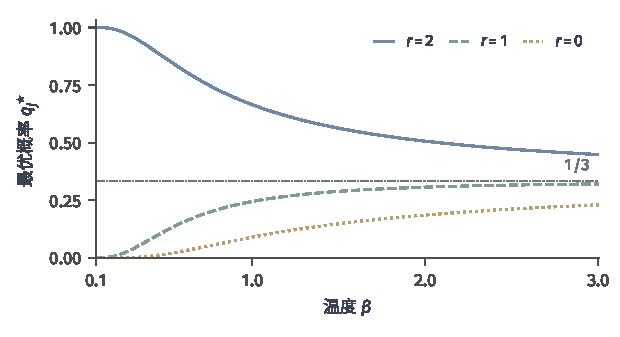
\includegraphics[width=105mm]{figures/00-shared/mathematical-preliminaries-lower/01-random-variables-distributions-and-causality/matplotlib/information-gibbs-temperature-weights/figure.pdf}
  \caption{三结果Gibbs分布随温度的变化。取\(P_0=(1/3,1/3,1/3)\)、收益\(r=(0,1,2)\)，曲线按\(q_j^\star(\beta)=e^{r_j/\beta}/\sum_k e^{r_k/\beta}\)计算；实线、虚线、点线分别对应收益\(2,1,0\)。灰点划线为参考概率\(1/3\)；\(\beta\downarrow0\)时质量集中到唯一最高收益结果，\(\beta\to\infty\)时恢复参考分布。}
  \label{fig:information-gibbs-temperature-weights}
\end{figure}

\subsubsection{矩约束下的最大熵选择}
\label{sec:information-maximum-entropy}

若只知道均值或协方差，没有指定收益函数，哪些分布与这些信息相容？
\term{最大熵原理}（maximum entropy principle）在相容分布中选择熵最大的一个。
它把“不过度集中”落实到一个明确的优化准则，不表示该分布已被观测证明为真；
参考测度和矩约束仍是建模选择。

骰子是可以手算的对照。没有任何矩信息时，六面等概率的熵最大，
为\(\log6\approx1.792\) nat；若已知平均点数为\(4.5\)而非默认的\(3.5\)，
等概率分布不再可行，最大熵解是指数倾斜的形式
\(p_k\propto e^{\lambda k}\)，其中\(\lambda\)由
\(\sum_kk e^{\lambda k}/\sum_k e^{\lambda k}=4.5\)确定；
数值求解得\(\lambda\approx0.371\)，六面概率自\(1\)到\(6\)依次约为
\(0.054,0.079,0.114,0.165,0.240,0.347\)，熵降到约\(1.614\) nat。
可见约束把概率推向高点，熵随之下降。反过来，只报告均值\(4.5\)而不报告分布时，
符合该均值的分布有很多。最大熵准则在其中选择熵最大的一个，
避免在这一准则下额外集中概率。随机结果的平均自信息在所选参考测度和矩约束下达到最大。
参考测度、矩约束和最大熵准则仍是建模选择，
不能据此断言真实骰子服从这个分布。

固定参考测度\(\mu\)，要求密度\(p\)满足
\[
  \int p\,\mathrm d\mu=1,\qquad
  \int \bm T(x)p(x)\,\mathrm d\mu(x)=\bm\tau.
\]
若存在有限参数\(\bm\lambda\)，使
\[
  p_{\bm\lambda}(x)
  =\exp\{\bm\lambda^\top\bm T(x)-A(\bm\lambda)\},\qquad
  A(\bm\lambda)=\log\int e^{\bm\lambda^\top\bm T(x)}\,\mathrm d\mu(x)<\infty
\]
归一化并满足这些矩约束，则它是最大熵的候选。
形式上，对熵加归一化和矩约束的Lagrange项，密度方向的一阶条件为
\(-\log p-1+\bm\lambda^\top\bm T+a=0\)，从而给出上述指数形式。
但这一步没有证明解存在，也没有处理所有无限维变分的合法性；
真正的最优性可由KL直接核验。

对任意同样可行、统计量可积且熵有限的密度\(p\)，若候选自身也满足这些有限性条件，
\[
\begin{aligned}
  D_{\mathrm{KL}}(p\Vert p_{\bm\lambda})
  &=\int p\log p\,\mathrm d\mu-\bm\lambda^\top\bm\tau+A(\bm\lambda)\\
  &=-h_\mu(p)+h_\mu(p_{\bm\lambda})\geq0.
\end{aligned}
\]
因此候选最大化熵，等号当且仅当两密度几乎处处相同。
矩约束不可达、配分函数无限或最大熵没有上界时，乘子方程不能弥补这些缺口。
即使最大熵分布存在，边界约束也可能只能由无穷自然参数的极限表示。

固定均值\(\bm m\)和正定协方差\(\bm\Sigma\)时，
\(q=\mathcal N(\bm m,\bm\Sigma)\)给出一个完整实例。
其对数密度为
\[
  \log q(\bm x)
  =-\frac d2\log(2\pi)-\frac12\log\det\bm\Sigma
   -\frac12(\bm x-\bm m)^\top\bm\Sigma^{-1}(\bm x-\bm m).
\]
任意具有同样均值和协方差的密度\(p\)都满足
\[
  \mathbb E_p[(\bm X-\bm m)^\top\bm\Sigma^{-1}(\bm X-\bm m)]
  =\operatorname{tr}(\bm\Sigma^{-1}\bm\Sigma)=d.
\]
因而\(\mathbb E_p\log q=\mathbb E_q\log q\)，在\(h(p)\)有限时，
\[
  D_{\mathrm{KL}}(p\Vert q)=h(q)-h(p)\geq0,\qquad
  h(p)\leq\frac12\log\{(2\pi e)^d\det\bm\Sigma\}.
\]
等号唯一对应高斯。这仍是在固定坐标和Lebesgue参考测度下比较微分熵。
协方差奇异时，分布被限制在低维仿射子空间，不能继续使用原空间中的密度公式；
须改用子空间参考测度。

指数形式还把分布优化与参数表示联系起来。
对前章的指数族
\[
  p_{\bm\eta}(x)
  =h(x)\exp\{\bm\eta^\top\bm T(x)-A(\bm\eta)\},
\]
在允许交换微分积分的自然参数内部，
\(\nabla A(\bm\eta)=\mathbb E_{\bm\eta}\bm T=\bm\tau\)，
\(\nabla^2A(\bm\eta)=\operatorname{Cov}_{\bm\eta}(\bm T)\)。
自然参数\(\bm\eta\)指定指数权重，均值参数\(\bm\tau\)指定统计量平均。

若反过来给定均值，要恢复哪一个指数权重？Bernoulli族给出一个可直接计算的例子。
在\(x\in\{0,1\}\)上取\(T(x)=x\)、\(h(x)=1\)，则\(A(\eta)=\log(1+e^\eta)\)，
\(\tau=A'(\eta)=e^\eta/(1+e^\eta)\)。给定\(0<\tau<1\)，解得
\(\eta=\log\{\tau/(1-\tau)\}\)。把它代入\(\eta\tau-A(\eta)\)，得到
\[
 \tau\log\tau+(1-\tau)\log(1-\tau),
\]
即Bernoulli分布的负熵。

一般情形未必能显式反解参数，但仍可固定均值\(\bm\tau\)，
对\(\bm\eta\)最大化\(\bm\eta^\top\bm\tau-A(\bm\eta)\)。
为记录这个最优值，定义配分函数的凸共轭
\begin{equation}
  A^\star(\bm\tau)
  =\sup_{\bm\eta}\{\bm\eta^\top\bm\tau-A(\bm\eta)\}.
  \label{eq:information-log-partition-conjugate}
\end{equation}
若\(\bm\tau=\nabla A(\bm\eta)\)由有限自然参数实现，凸性的一阶不等式给出
\(A(\bm\zeta)\geq A(\bm\eta)+\bm\tau^\top(\bm\zeta-\bm\eta)\)。
移项可知共轭上确界在\(\bm\eta\)达到，且
\[
  A^\star(\bm\tau)=\bm\eta^\top\bm\tau-A(\bm\eta)
  =\int p_{\bm\eta}\log\frac{p_{\bm\eta}}h\,\mathrm d\mu.
\]
最后一个量是相对于基准项\(h\)的负熵；若\(h\)本身为概率密度，它就是KL。
只有\(h=1\)时才能直接写成普通负熵。
相关工具可参考\BookChapterRef{chap:optimization}{卷1《数学准备：计算、分析与几何》的“最优化”章}。

两组参数能否在局部互换，还取决于统计量有无冗余。所谓最小表示，是指不存在非零向量
\(\bm a\)，使\(\bm a^\top\bm T(x)\)在基准测度\(h\,\mathrm d\mu\)下几乎处处为常量。
在自然参数空间的开内部，这个条件给出
\[
 \bm a^\top\operatorname{Cov}_{\bm\eta}(\bm T)\bm a
 =\operatorname{Var}_{\bm\eta}(\bm a^\top\bm T)>0
 \qquad(\bm a\neq\bm0),
\]
因为有限自然参数的指数因子严格为正，模型分布与基准测度具有相同的零测集。
所以协方差正定，\(\mathrm d\bm\tau=\nabla^2A\,\mathrm d\bm\eta\)的Jacobian可逆，
由逆函数定理可得两组参数局部一一对应。
若统计量有含常量项的仿射冗余，例如某一坐标恒为\(1\)，协方差就会奇异；
只排除不同统计量之间的线性组合还不够。

有限配置可以不预设每个均值都由有限参数实现，而直接覆盖闭可行域。
\begin{theorem}[有限配置上的配分函数与最大熵对偶]
\label{thm:information-finite-entropy-duality}
设\(D\)为有限非空配置集，\(\bm T:D\to\mathbb R^m\)，基准权重恒为\(1\)。
定义
\[
  A(\bm\theta)=\log\sum_{z\in D}e^{\langle\bm\theta,\bm T(z)\rangle},
  \qquad\mathcal M=\operatorname{conv}\{\bm T(z):z\in D\}.
\]
对\(\bm\mu\in\mathcal M\)，令
\[
  H^\star(\bm\mu)=\max_{q:\,\mathbb E_q\bm T=\bm\mu}H(q),
\]
其中\(q\)遍历\(D\)上的全部概率质量函数。则在整个\(\mathcal M\)上有
\(A^\star(\bm\mu)=-H^\star(\bm\mu)\)，在外部有\(A^\star=+\infty\)，且
\begin{equation}
  A(\bm\theta)=\max_{\bm\mu\in\mathcal M}
  \{\langle\bm\theta,\bm\mu\rangle+H^\star(\bm\mu)\}.
  \label{eq:information-finite-gibbs-duality}
\end{equation}
\end{theorem}
\begin{proof}
有限概率单纯形紧；给定可行均值后的约束闭且非空，熵在单纯形上连续，
因此每个\(H^\star(\bm\mu)\)都能达到。
令\(p_{\bm\theta}(z)=e^{\langle\bm\theta,\bm T(z)\rangle-A(\bm\theta)}\)。
对任意质量函数\(q\)，展开有限KL得到
\[
  \langle\bm\theta,\mathbb E_q\bm T\rangle+H(q)
  =A(\bm\theta)-D_{\mathrm{KL}}(q\Vert p_{\bm\theta})
  \leq A(\bm\theta),
\]
且在\(q=p_{\bm\theta}\)处取等号。把所有\(q\)按均值分组，
组内线性项相同，只需保留最大熵者，即得式~\eqref{eq:information-finite-gibbs-duality}。

为证明边界处也有共轭等式，在\(\mathcal M\)上令\(f=-H^\star\)，
在外部令\(f=+\infty\)。
取两个均值及其最大熵分布\(q_1,q_2\)，混合
\(tq_1+(1-t)q_2\)的均值为对应均值的凸组合。
熵凹性给出
\[
  H^\star(t\bm\mu_1+(1-t)\bm\mu_2)
  \geq H(tq_1+(1-t)q_2)
  \geq tH^\star(\bm\mu_1)+(1-t)H^\star(\bm\mu_2).
\]
所以\(f\)凸。
若\(\bm\mu_n\to\bm\mu\)且各均值可行，先取使最大熵值趋于上极限的子列，
再从对应的最大熵分布中取收敛子列\(q_{n_k}\to q\)。
有限维均值映射连续，故\(\mathbb E_q\bm T=\bm\mu\)；熵连续性给出
\[
  \limsup_nH^\star(\bm\mu_n)=H(q)\leq H^\star(\bm\mu).
\]
于是\(H^\star\)上半连续。又因\(\mathcal M\)闭，
扩展后的\(f\)在整个\(\mathbb R^m\)上下半连续。
由\(0\leq H^\star\leq\log|D|\)和\(\mathcal M\neq\varnothing\)，
\(f\)适当。前半证明已说明\(f^\star=A\)。适当下半连续凸函数等于自身的双共轭，因而
\(A^\star=f^{\star\star}=f\)，包括边界均值和可行域外部。
此证明不要求共轭上确界由有限自然参数达到。
\end{proof}

\(\mathcal M\)是可实现统计量均值的凸包。
统计量由各局部配置的指示函数组成时，它称为边缘多面体；
属于该集合表示局部概率表能同时来自同一全局分布，
强于每张表单独归一化。例如两个二元变量的两张边缘表均令取值\(1\)的概率为\(0.1\)，
则联合表不可能同时要求\(P(X=1,Y=1)=0.9\)。
局部数字各自在\([0,1]\)内，并不足以保证共同可实现。

在\(\{0,1,2\}\)上要求\(\mathbb EX=1/2\)时，最大熵分布为
\(p_j=t^j/(1+t+t^2)\)。均值方程给出
\[
  \frac{t+2t^2}{1+t+t^2}=\frac12,\qquad
  3t^2+t-1=0,\qquad
  t=\frac{\sqrt{13}-1}{6}\approx0.4343.
\]
故\((p_0,p_1,p_2)\approx(0.6162,0.2676,0.1162)\)。
自然参数是\(\lambda=\log t\)，
\(H(p)=\log(1+t+t^2)-\lambda/2\)，与共轭负熵一致。
若均值改为边界值\(0\)，唯一可行分布为\(\delta_0\)，熵为零；
它由\(t\downarrow0\)、\(\lambda\to-\infty\)逼近，却没有有限自然参数表示。
这正是分布最优解存在与有限参数实现之间的区别。

\subsection{表示约束下的分布逼近}
\label{sec:information-elbo-approximation}

联合模型与固定观测可以确定隐变量的后验密度：保留隐变量\(z\)作为自变量，把联合密度\(p_{\bm\theta}(x,z)\)除以归一化常数\(p_{\bm\theta}(x)\)。对全部隐变量积分得到的是这个常数，即模型证据，而不是仍以\(z\)为自变量的后验。在复杂模型中，证据积分可能难以解析或数值计算；对于多个离散隐变量，其联合配置数还可能随变量数指数增长。变分推断于是从可计算候选族中选择密度\(q\)，以指定方向的KL逼近已经由模型确定的后验。固定观测\(x\)和模型参数\(\bm\theta\)，设
\[
  0<p_{\bm\theta}(x)=\int p_{\bm\theta}(x,z)\,\mathrm dz<\infty,
  \qquad
  \pi(z)=p_{\bm\theta}(z\mid x).
\]
记候选密度为\(q\)。证据积分可能难算，候选\(q\)则允许采样和评价密度。

直接最小化\(q\)到后验\(\pi\)的KL，仍会遇到\(\pi\)中难算的证据常数。这个常数不随\(q\)改变，因而可以把含它的部分与可计算部分分开：用候选\(q\)抽样，只评价联合密度与\(q\)自身的对数比。下面的证据下界就是这一可计算目标；后面的恒等式说明最大化它为何等价于最小化该方向的KL。
\begin{definition}[证据下界]
\label{def:information-elbo}
若\(q\ll\pi\)且\(D_{\mathrm{KL}}(q\Vert\pi)<\infty\)，定义
\term{证据下界}（evidence lower bound, ELBO）为
\[
  \mathcal L(q,\bm\theta;x)
  =\mathbb E_q\log\frac{p_{\bm\theta}(x,Z)}{q(Z)}.
\]
按对数比整体取期望，不要求\(\mathbb E_q\log p_{\bm\theta}(x,Z)\)
与\(\mathbb E_q\log q(Z)\)各自有限。
\end{definition}

有限KL保证上述整体对数比可积，因为它等于
\(\log p_{\bm\theta}(x)-\log(q/\pi)\)。
直接分解就得到
\begin{equation}
  \log p_{\bm\theta}(x)
  =\mathcal L(q,\bm\theta;x)+D_{\mathrm{KL}}(q\Vert p_{\bm\theta}(\cdot\mid x)).
  \label{eq:information-elbo-decomposition}
\end{equation}
因此它确为下界，等号当且仅当\(q=\pi\)。
若KL无限，可以把ELBO扩展为\(-\infty\)，
但应使用\(\mathcal L=\log p_{\bm\theta}(x)-D_{\mathrm{KL}}\)这一方向，
不把右侧的\(-\infty+\infty\)当作合法分解。

另一条常见推导先乘除\(q\)，再使用Jensen不等式。
这里重要性等号需要相反方向的覆盖条件\(\pi\ll q\)，
保证联合密度的正质量区域不会被\(q\)漏掉。
若同时满足\(\pi\ll q\)、\(q\ll\pi\)及\(D_{\mathrm{KL}}(q\Vert\pi)<\infty\)，则
\begin{align}
  \log p_{\bm\theta}(x)
  &=\log\mathbb E_q\left[\frac{p_{\bm\theta}(x,Z)}{q(Z)}\right]\notag\\
  &\geq\mathbb E_q\log\frac{p_{\bm\theta}(x,Z)}{q(Z)}
   =\mathcal L(q,\bm\theta;x).
  \label{eq:information-elbo-jensen}
\end{align}
只满足\(q\ll\pi\)时，KL分解仍成立，
但重要性期望实际为\(p_{\bm\theta}(x)\pi(\{q>0\})\)，可能小于证据。
例如\(\pi=(1/2,1/2)\)、\(q=(1,0)\)，KL为\(\log2\)，
ELBO是\(\log p_{\bm\theta}(x)-\log2\)，而重要性期望只恢复一半证据。
反过来，若\(\pi=(1,0)\)、\(q=(1/2,1/2)\)，虽完整覆盖目标，
但\(q\)在零后验区域放了质量，反向KL无限。两种支持要求不能互相代替。

表~\ref{tab:information-candidate-support}将支持方向与两种计算并列。完整恢复证据要求候选覆盖后验，
而有限的\(D_{\mathrm{KL}}(q\Vert\pi)\)还要求候选不在零后验区域放置质量；两者控制的对象不同。
\begin{table*}[htbp]
  \centering\small
  \begin{tabularx}{\linewidth}{XXcccc}
    \toprule
    后验\(\pi\) & 候选\(q\) & \(q\ll\pi\) & \(\pi\ll q\) & \(D_{\mathrm{KL}}(q\Vert\pi)\) & 证据恢复比例\\
    \midrule
    \((1/2,1/2)\) & \((1,0)\) & 是 & 否 & \(\log2\) & \(1/2\)\\
    \((1,0)\) & \((1/2,1/2)\) & 否 & 是 & \(+\infty\) & \(1\)\\
    \((1/2,1/2)\) & \((1/2,1/2)\) & 是 & 是 & \(0\) & \(1\)\\
    \bottomrule
  \end{tabularx}
  \caption{候选支持对KL与证据恢复的影响。两点分布共用同一取值集合，证据满足
  \(0<p_{\bm\theta}(x)<\infty\)。恢复比例为\(\mathbb E_q[p_{\bm\theta}(x,Z)/q(Z)]/p_{\bm\theta}(x)=\pi(\{q>0\})\)，
  比值仅在\(q>0\)处评价。表中的有限KL是具体例子的结果；一般空间中\(q\ll\pi\)不能单独保证KL有限。}
  \label{tab:information-candidate-support}
\end{table*}

固定模型后最大化ELBO，等价于在候选族\(\mathcal Q\)中最小化
\(D_{\mathrm{KL}}(q\Vert\pi)\)。
假设\(\mathcal Q\)中至少有一个有限KL的候选，并且实际候选\(q\)也具有有限KL。
此时族内下确界是有限的非负数，实际候选的KL可写为
\[
  D_{\mathrm{KL}}(q\Vert\pi)
  =\inf_{\widetilde q\in\mathcal Q}D_{\mathrm{KL}}(\widetilde q\Vert\pi)
   +\left[D_{\mathrm{KL}}(q\Vert\pi)
    -\inf_{\widetilde q\in\mathcal Q}D_{\mathrm{KL}}(\widetilde q\Vert\pi)\right].
\]
第一项是表示限制，第二项是未达到族内最优的求解误差。
在上述有限性条件下，即使最优候选不存在，这个按下确界的分解仍有效。
若候选族中的KL全部无限，就没有有限ELBO候选，不能用无穷减无穷定义求解误差。
若同时拟合\(\bm\theta\)，证据和后验也随之改变，
模型与真实观测分布的拟合误差是另一层问题，不等于这两项之和。

取\(Z\sim\mathcal N(0,1)\)、\(X\mid Z\sim\mathcal N(Z,1)\)，观测\(x=1\)。
配平方得到后验\(Z\mid X=1\sim\mathcal N(1/2,1/2)\)。
边缘上\(X\sim\mathcal N(0,2)\)，证据\(p(x)\)是这个边缘密度在\(x=1\)处的值。
若\(q=\mathcal N(0,1)\)，
\[
\begin{aligned}
  \log p(x)&=-\tfrac12\log(4\pi)-\tfrac14\approx-1.5155,\\
  D_{\mathrm{KL}}(q\Vert\pi)
  &=\tfrac12\{2+\tfrac12-1+\log(1/2)\}\approx0.4034,\\
  \mathcal L(q;x)&\approx-1.9189.
\end{aligned}
\]
三者满足精确分解。多变量情形把\(q\)限制为分块独立族，
可能留下无法表示的后验相关性；求解更充分也不能消除这一表示限制。

分布蒸馏采用另一个给定目标：教师的条件分布\(P_{\mathrm T}(\cdot\mid x)\)。
在有限类别空间和固定输入权重下，最小化条件KL的平均
\(\mathbb E_XD_{\mathrm{KL}}(P_{\mathrm T}(\cdot\mid X)\Vert Q_{\bm\phi}(\cdot\mid X))\)
等价于教师软标签下的交叉熵，要求学生覆盖教师的正质量类别。
反向KL改由学生平均，支持要求和最优近似都会改变。
学生逼近教师，不自动意味着更接近真实标签规律。

前面的互信息比较\(P_{XY}\)与\(P_X\otimes P_Y\)。现在把联合配对样本与若干独立边缘样本放进同一候选组，待逼近的对象改为给定这组观测后正样本位置的后验概率。评分函数通过有限候选上的归一化表示这张后验；能否恢复它，取决于评分函数类和候选的抽样规律。
以信息噪声对比估计（information noise-contrastive estimation, InfoNCE）损失为例，取总候选数\(K\geq2\)，按目标联合分布抽取
\((X,Y_1)\)，再独立地按边缘\(P_Y\)抽取\(Y_2,\ldots,Y_K\)；
这些负样本彼此独立，也独立于\((X,Y_1)\)。对可测实值评分函数\(s\)，定义
\begin{equation}
 \mathcal L_K
 =\mathbb E\left[-\log
   \frac{\exp s(X,Y_1)}{\sum_{j=1}^K\exp s(X,Y_j)}\right].
 \label{eq:information-contrastive-loss}
\end{equation}
它把相对评分归一化为候选类别概率，再惩罚未能认出正样本的预测。
\(K\)包括一个正样本和\(K-1\)个负样本；期望针对上述全部抽样。
若该损失可积，则
\[
 \log K-\mathcal L_K\leq I(X;Y).
\]

这个下界可分两步推得：先将分类损失与观测提供的正样本位置信息联系起来，
再说明这部分信息不超过目标变量之间的互信息。
我们使用等价的抽样方式，将正样本位置也随机化：先在\(K\)个位置中均匀选择\(J\)，
令该位置与\(X\)按目标联合分布配对，其余位置仍为独立边缘样本。
记整组观测为\(W=(X,Y_1,\ldots,Y_K)\)。

图~\ref{fig:information-contrastive-hidden-position}把\(K=3\)时的一次生成安排画开：示意中恰好抽到\(J=2\)，所以只有\(Y_2\)与\(X\)按目标联合规律配对，其余两个候选各自按边缘规律独立抽取。图中的位置标记供我们核对生成规则；实际识别位置时，观察者只得到\(W\)，并不知道\(J\)。因此需要预测的是“这组候选中哪个位置由联合规律生成”，而不是直接把整组候选当成从\(P_{Y\mid X}\)独立抽来的结果。

\begin{figure*}[htbp]
  \centering
  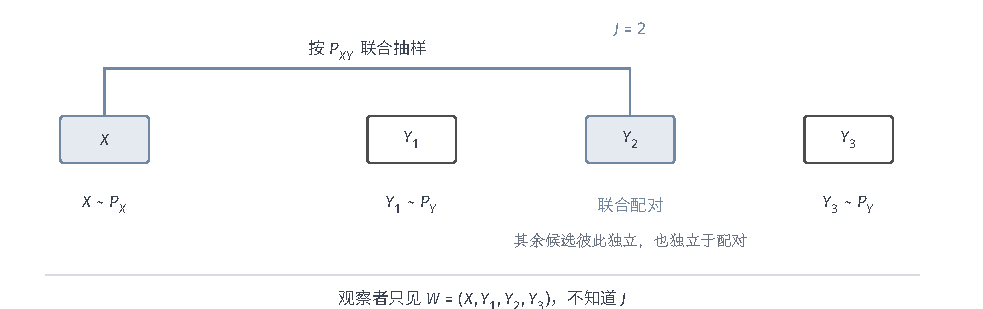
\includegraphics[width=169mm]{figures/00-shared/mathematical-preliminaries-lower/01-random-variables-distributions-and-causality/tikz/information-contrastive-hidden-position/source.pdf}
  \caption{InfoNCE的隐藏正样本位置。图示总候选数为\(K=3\)，均匀抽取的位置在这一次为\(J=2\)。蓝色连线连接按\(P_{XY}\)联合抽取的\((X,Y_2)\)；其余候选彼此独立，也独立于这一配对，并按\(P_Y\)抽取。连线表达抽样依赖，图中不是因果生成结构；识别者看到的整组观测\(W\)不包含位置标签\(J\)。}
  \label{fig:information-contrastive-hidden-position}
\end{figure*}

同一个评分规则在各位置对称使用，所以平均分类损失仍为\(\mathcal L_K\)。记评分给出的类别概率为
\[
 q_s(j\mid W)=\frac{\exp s(X,Y_j)}{\sum_{u=1}^K\exp s(X,Y_u)}.
\]

可以进一步写清它要逼近的真实位置后验。若\(I(X;Y)<\infty\)，联合分布对边缘乘积绝对连续，记密度比为
\(r(x,y)=\mathrm dP_{XY}/\mathrm d(P_X\otimes P_Y)(x,y)\)。固定\(J=j\)时，整组观测相对完全独立规律的密度比只有\(r(X,Y_j)\)这一项；其余候选的边缘因子均相同。因此均匀位置先验与Bayes公式给出
\[
 P(J=j\mid W)
 =\frac{r(X,Y_j)}{\sum_{u=1}^K r(X,Y_u)},
 \qquad P_W\text{几乎处处}.
\]
分母在整组观测的真实规律下几乎处处为正。归一化评分\(q_s\)是在逼近这张位置后验；评分函数能否表示所需的相对权重，仍是候选表示的限制。这个表达式还明确了为什么必须保留负样本的独立边缘抽样约定：更换那项约定，真实位置后验的密度比也会改变。
有限实值评分使各类别概率严格为正。按真实位置后验计算交叉熵，并使用式~\eqref{eq:information-cross-entropy-decomposition}，得到
\[
 \mathcal L_K=H(J\mid W)+\mathbb E_W D_{\mathrm{KL}}\bigl(P_{J\mid W}\Vert q_s(\cdot\mid W)\bigr).
\]
这里\(H(J\mid W)\leq\log K\)，且假设分类损失可积，因此两项都有限。第二项明确度量评分表示对位置后验的逼近误差；其非负性也给出后面所需的熵下界。因此
\[
 \log K-\mathcal L_K\leq H(J)-H(J\mid W)=I(J;W).
\]

还需说明识别正样本位置的信息不会超过目标互信息。令\(P_j\)为给定\(J=j\)的
\(W\)分布，\(M=K^{-1}\sum_jP_j\)，并以完全独立规律
\(Q=P_X\otimes P_Y^{\otimes K}\)作参照。若\(I(X;Y)<\infty\)，
每个\(P_j\)相对于\(Q\)只有正样本配对这一项密度比，所以
\[
\begin{aligned}
 I(X;Y)&=\frac1K\sum_{j=1}^KD_{\mathrm{KL}}(P_j\Vert Q)\\
 &=\frac1K\sum_{j=1}^KD_{\mathrm{KL}}(P_j\Vert M)
      +D_{\mathrm{KL}}(M\Vert Q)\\
 &=I(J;W)+D_{\mathrm{KL}}(M\Vert Q)\geq I(J;W).
\end{aligned}
\]
中间等式将对数密度比拆成经过\(M\)的两项，再对\(j\)平均；
互信息无限时原下界自动成立。

又因分类损失非负，\(\log K-\mathcal L_K\leq\log K\)，
有限候选数确实会限制这个下界的最大数值。
不符合采样假设时，不能把优化该分类目标直接解释为增加原分布的互信息；
即使下界合法，也不自动保证校准、语义质量或下游风险。

\subsection{边缘约束下的分布耦合}
\label{sec:information-coupling-optimization}

把两个固定边缘\(P,Q\)配成联合分布时，可以有许多不同的配对。未知量是
\(\gamma\in\Pi(P,Q)\)，每个候选都须保留这两个边缘。给出位置之间的搬运成本后，最优配对决定哪些质量配到哪些位置。独立乘积说明可行集合非空，但它未必使平均成本最小。
定义~\ref{def:information-coupling}与式~\eqref{eq:information-kantorovich-transport}
已经给出可行集合和成本，这里补足最小值的存在与有限求解。

\subsubsection{边缘约束下的最优耦合存在}
\label{sec:information-optimal-coupling-existence}

一般空间中的测度序列可能把质量送往越来越远处，存在性证明因而需要排除质量逃逸。
在当前耦合问题中，固定边缘的紧性将给出对全部可行耦合统一适用的紧集。
有了这一控制，还要保住极限的两侧边缘，并使极限成本不增加。
第~\ref{sec:rv-weak-convergence}节的概率测度弱收敛及紧性正好服务这三步。
这里不重新定义它们：变化对象是乘积空间上的概率测度，
测试函数是有界连续函数；这不同于泛函分析中固定线性空间内由连续线性泛函
检验的弱拓扑。二者都有“弱收敛”这一中文名称，但不能不说明对象就互换结论。

\begin{theorem}[最优耦合存在]
\label{thm:information-optimal-coupling-existence}
设\(\mathcal X,\mathcal Y\)为Polish空间，\(P,Q\)为其Borel概率测度。
若成本\(c:\mathcal X\times\mathcal Y\to[0,\infty]\)下半连续，
且至少有一个\(\gamma_0\in\Pi(P,Q)\)满足\(\int c\,\mathrm d\gamma_0<\infty\)，
则存在有限成本耦合\(\gamma^\star\)达到
\(\mathcal T_c(P,Q)=\inf_{\gamma\in\Pi(P,Q)}\int c\,\mathrm d\gamma\)。
\end{theorem}
\begin{proof}
可行集合非空，且成本非负、有有限可行值，所以最优下确界有限。
取近最优序列\(\gamma_n\in\Pi(P,Q)\)，使
\(\int c\,\mathrm d\gamma_n\to\mathcal T_c(P,Q)\)。

Polish空间上的Borel概率测度紧。
任给\(\varepsilon>0\)，分别选择紧集\(K_{\mathcal X},K_{\mathcal Y}\)，使
\(P(K_{\mathcal X}^{\mathsf c})<\varepsilon/2\)、
\(Q(K_{\mathcal Y}^{\mathsf c})<\varepsilon/2\)。
其乘积紧，且任意可行耦合都满足
\[
  \gamma((K_{\mathcal X}\times K_{\mathcal Y})^{\mathsf c})
  \leq P(K_{\mathcal X}^{\mathsf c})+Q(K_{\mathcal Y}^{\mathsf c})
  <\varepsilon.
\]
因边缘固定，这个紧集对全部\(\gamma\)同时适用，
从而\((\gamma_n)\)一致紧。
乘积空间仍为Polish空间，定理~\ref{thm:rv-prokhorov}给出子列
\(\gamma_{n_k}\Rightarrow\gamma^\star\)。

对任意有界连续\(a:\mathcal X\to\mathbb R\)，函数
\((x,y)\mapsto a(x)\)有界连续，故
\[
  \int a(x)\,\mathrm d\gamma^\star(x,y)
  =\lim_k\int a(x)\,\mathrm d\gamma_{n_k}(x,y)=\int a\,\mathrm dP.
\]
有界连续函数区分Borel概率测度，因此\(\gamma^\star\)的第一边缘为\(P\)。
同理第二边缘为\(Q\)，所以极限仍可行。

最后，对非负下半连续成本使用定理~\ref{thm:rv-portmanteau}：
\[
  \int c\,\mathrm d\gamma^\star
  \leq\liminf_k\int c\,\mathrm d\gamma_{n_k}
  =\mathcal T_c(P,Q).
\]
可行性又给出反向不等式，所以等号成立且成本有限。
\end{proof}

最后一步的积分测度随\(k\)改变，不能用固定测度下的Fatou引理直接替代。
非负性避免成本的负部失控，下半连续性保证极限不会突然增加成本；
若修改这些假设，需要另给能实现同样作用的条件。
存在联合耦合也不保证存在确定搬运映射。
例如\(P=\delta_0\)、\(Q=(\delta_{-1}+\delta_1)/2\)时，
唯一来源点必须把质量分成两半，任何单值映射都只能把它送到一个点。

\subsubsection{有限空间下的最优耦合求解}
\label{sec:information-finite-transport}

设来源点为\(x_i\)、目标点为\(y_j\)，概率向量为\(\bm p,\bm q\)，
各成本\(c_{i,j}\)有限且非负。搬运表\(\bm\gamma\)的行和是来源质量，
列和是目标质量，问题为
\[
  \min_{\gamma_{i,j}\geq0}\sum_{i,j}c_{i,j}\gamma_{i,j},
  \qquad \sum_j\gamma_{i,j}=p_i,\quad\sum_i\gamma_{i,j}=q_j.
\]
独立表\(\gamma_{i,j}=p_iq_j\)可行。
约束集合闭，且每个元素在\([0,1]\)内，因此它是紧多面体，
线性目标可以取到最小值。

把有限搬运视为线性规划，并为两组边缘约束引入势函数
\(u_i,v_j\)，保留\(\gamma_{i,j}\geq0\)作为取下确界的定义域：
\begin{align}
  \mathcal L(\bm\gamma,\bm u,\bm v)
  &=\sum_{i,j}c_{i,j}\gamma_{i,j}
    +\sum_i u_i\left(p_i-\sum_j\gamma_{i,j}\right)
    +\sum_j v_j\left(q_j-\sum_i\gamma_{i,j}\right)\notag\\
  &=\sum_i u_ip_i+\sum_jv_jq_j
    +\sum_{i,j}(c_{i,j}-u_i-v_j)\gamma_{i,j}.
  \label{eq:information-discrete-ot-lagrangian}
\end{align}
如果某个系数\(c_{i,j}-u_i-v_j<0\)，将对应非负变量趋向无穷，
Lagrangian下确界就是\(-\infty\)。
若全部系数非负，下确界可在\(\bm\gamma=\bm0\)取到，
值为\(\sum_i u_ip_i+\sum_jv_jq_j\)。
这里消元时边缘等式已进入Lagrangian，不再限制\(\bm\gamma\)，
所以零表虽不是原问题的可行表，却可以用于计算对偶函数。
于是
\[
  g(\bm u,\bm v)=
  \begin{cases}
    \sum_i u_ip_i+\sum_jv_jq_j,&u_i+v_j\leq c_{i,j}\text{ 对所有 }i,j,\\
    -\infty,&\text{否则}.
  \end{cases}
\]
最大化它得到
\begin{equation}
  \max_{\bm u,\bm v}
  \left\{\sum_i u_ip_i+\sum_jv_jq_j:\ u_i+v_j\leq c_{i,j}\right\}.
  \label{eq:information-discrete-ot-dual}
\end{equation}
势函数约束来自消元后下确界有限的必要充分条件，不是额外猜出的搬运规则。
对任意原始可行表，将\(u_i+v_j\leq c_{i,j}\)逐项乘\(\gamma_{i,j}\)
并求和，立刻得到对偶值不超过搬运成本。
有限维原问题可行且最优值有限，线性规划强对偶又保证两者最优值相等。

取来源和目标位置均为\(0,2\)，令\(\bm p=(3/4,1/4)\)、\(\bm q=(1/4,3/4)\)，
\(c_{i,j}=|x_i-y_j|\)。全部可行表都能写成
\[
  \bm\gamma(a)=
  \begin{pmatrix}
    a&3/4-a\\
    1/4-a&a
  \end{pmatrix},\qquad 0\leq a\leq1/4.
\]
对角线成本为零，两个非对角线成本均为\(2\)，
故总成本为\(2-4a\)，在\(a=1/4\)处最小：
\[
  \bm\gamma^\star=
  \begin{pmatrix}1/4&1/2\\0&1/4\end{pmatrix},\qquad
  \sum_{i,j}c_{i,j}\gamma^\star_{i,j}=1.
\]
对偶取\(\bm u=(0,-2)\)、\(\bm v=(0,2)\)，四项和依次为
\(0,2,-2,0\)，均不超过对应成本\(0,2,2,0\)。
对偶值为
\[
  \bm u^\top\bm p+\bm v^\top\bm q
  =-2(1/4)+2(3/4)=1.
\]
弱对偶已足以核验最优性：所有可行表成本至少为\(1\)，而上表恰好达到。
图~\ref{fig:information-transport-tables}比较这个表与独立配对，
说明相同行列边缘不能决定搬运成本。
\begin{figure}[htbp]
  \centering
  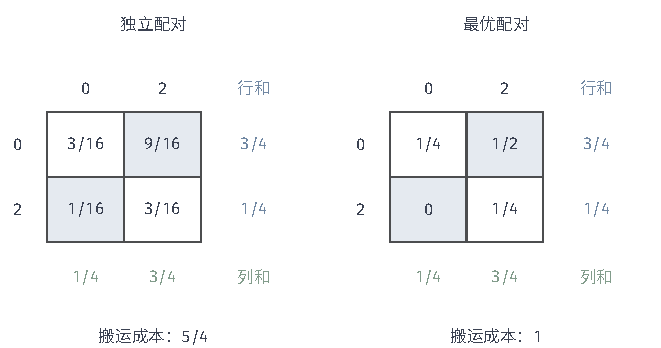
\includegraphics[width=\linewidth]{figures/00-shared/mathematical-preliminaries-lower/01-random-variables-distributions-and-causality/tikz/information-transport-tables/figure.pdf}
  \caption{同一边缘约束下的两张搬运表。来源和目标都位于\(0,2\)，
  蓝色行和为\(\bm p=(3/4,1/4)\)，绿色列和为\(\bm q=(1/4,3/4)\)。
  浅色单元格承担非零距离成本。独立表的成本为\(5/4\)，最优表为\(1\)；
  正文的势函数给出与最优表相等的对偶值。}
  \label{fig:information-transport-tables}
\end{figure}

\section{参数化概率分布的几何与优化}
\label{sec:information-global-local-geometry}
\label{sec:information-fisher-geometry}

前面的分布选择、逼近和耦合都可以通过候选参数来求解；参数表示须保留各自的可行约束。设当前候选族为\(\{P_{\bm\theta}:\bm\theta\in\Theta\}\)。到目前为止，比较分布差异用的都是KL、TV等不依赖参数坐标的量。现在回到用参数表示的模型族：当算法沿某个参数方向更新一步时，怎样度量这一步在“分布空间”里走了多远？欧氏距离\(\|\bm\delta\|_2\)并不合适——同样的参数位移，在噪声很小的模型里会让分布面目全非，在噪声很大时却几乎看不出区别；而且参数的单位（秒还是毫秒、概率还是logit）可以任意改换，距离不应随之改变。
因此需要根据分布自身定义局部步长：先看一个无穷小参数扰动造成多少KL变化，再把这个二次变化量当作参数空间的内积。
本节回用优化与流形中的切向量、度量工具，但度量由概率模型的局部KL建立。
若参数化没有自动满足矩或边缘约束，仍要显式处理可行域，不能直接作无约束更新。

\subsection{参数变化下的分布距离}
\label{sec:information-local-metric}

改变参数值通常会改变分布；更换表示同一分布的坐标则不应该改变几何对象。
先分析前一种真实扰动，再检查后一种坐标变化。
我们先用对数密度的参数导数记录各方向的局部敏感性，再对这些导数的外积取平均，得到分布自身决定的局部尺度。

\paragraph{参数敏感性与Fisher信息}
\term{Fisher信息}（Fisher information）衡量观测分布对参数局部变化的敏感程度。

\begin{definition}[Fisher信息矩阵]
\label{def:information-fisher-matrix}
对开参数域上的受共同测度支配模型\(p_{\bm\theta}\)，固定参数内点\(\bm\theta\)。假设在\(P_{\bm\theta}\)-几乎每个\(x\)处，\(p_{\bm\theta}(x)>0\)且\(\log p_{\bm\theta}(x)\)关于参数可微。定义得分向量\(\bm s_{\bm\theta}(x)=\nabla_{\bm\theta}\log p_{\bm\theta}(x)\)；若\(\mathbb E_{\bm\theta}\lVert\bm s_{\bm\theta}(X)\rVert_2^2<\infty\)，该点的\term{Fisher信息矩阵}定义为
\begin{equation}
  \bm{F}(\bm{\theta})
  =
  \mathbb{E}_{\bm{\theta}}\!\left[
    \bm{s}_{\bm{\theta}}(X)
    \bm{s}_{\bm{\theta}}(X)^{\top}
  \right].
  \label{eq:information-fisher-matrix}
\end{equation}
它是得分外积在模型分布下的平均，必为半正定矩阵。标量参数时退化为得分平方的期望；这个定义本身不要求它等于负对数似然的期望Hessian，后一个恒等式还需正则条件。
\end{definition}

\paragraph{小参数变化下的分布差异}
\label{sec:information-local-kl}

设参数域\(\Theta\subseteq\mathbb R^d\)，共同参考测度为\(\mu\)。
固定内点\(\bm\theta\)，假设存在开邻域\(U\)和共同可测支持\(S\)，
使所有\(\bm\eta\in U\)都在\(S\)上满足\(p_{\bm\eta}>0\)，在外部为零。
再假设\(p_{\bm\eta}(x)\)对参数二阶连续可微，
其一、二阶导数分别由\(\mu\)-可积函数在\(U\)上一致控制。
这些条件允许对归一化等式交换一、二阶微分和积分。
沿用得分记号\(\bm s_{\bm\theta}(x)=\nabla_{\bm\theta}\log p_{\bm\theta}(x)\)，有
\begin{equation}
  \mathbb E_{\bm\theta}\bm s_{\bm\theta}(X)
  =\int\nabla_{\bm\theta}p_{\bm\theta}(x)\,\mathrm d\mu(x)=\bm0.
  \label{eq:information-score-zero}
\end{equation}

进一步要求
\[
  \mathbb E_{\bm\theta}\|\bm s_{\bm\theta}(X)\|_2^2<\infty,\qquad
  \mathbb E_{\bm\theta}
  \|\nabla^2_{\bm\theta}\log p_{\bm\theta}(X)\|_{\mathrm{op}}<\infty.
\]
此时Fisher矩阵
\(\bm F(\bm\theta)=\mathbb E_{\bm\theta}[\bm s_{\bm\theta}\bm s_{\bm\theta}^\top]\)
有限。乘积法则给出
\[
  \nabla^2_{\bm\theta}p_{\bm\theta}
  =p_{\bm\theta}
   \{\nabla^2_{\bm\theta}\log p_{\bm\theta}
      +\bm s_{\bm\theta}\bm s_{\bm\theta}^\top\}.
\]
两边积分，左侧由二阶微分归一化等式为零，故
\begin{equation}
  \bm F(\bm\theta)
  =-\mathbb E_{\bm\theta}\nabla^2_{\bm\theta}\log p_{\bm\theta}(X).
  \label{eq:information-fisher-hessian-identity}
\end{equation}
这就是此处使用的信息恒等式。
不能只对得分的零均值求导而忽略积分权重\(p_{\bm\theta}\)也依赖参数。
共同支持同样重要：例如均匀族\(\operatorname{Unif}(0,\theta)\)
有移动边界，内部对数密度导数为\(-1/\theta\)，其均值不为零；
这不反驳恒等式，而是没有满足推导条件。

\begin{theorem}[KL的局部二阶展开]
\label{thm:information-kl-local-fisher}
在上述共同支持、交换微分及可积条件下，进一步设\(U\)可取为凸集，
且对\(P_{\bm\theta}\)-几乎处处的\(x\)，
\(\nabla^2_{\bm\eta}\log p_{\bm\eta}(x)\)在\(\bm\theta\)处连续。
假设存在\(M\in L^1(P_{\bm\theta})\)，使
\[
  \sup_{\bm\eta\in U}
  \|\nabla^2_{\bm\eta}\log p_{\bm\eta}(x)\|_{\mathrm{op}}\leq M(x)
\]
几乎处处成立。则当\(\bm\delta\to\bm0\)且\(\bm\theta+\bm\delta\in U\)时，
\begin{equation}
  D_{\mathrm{KL}}(P_{\bm\theta}\Vert P_{\bm\theta+\bm\delta})
  =\tfrac12\bm\delta^\top\bm F(\bm\theta)\bm\delta
   +o(\|\bm\delta\|_2^2).
  \label{eq:information-kl-fisher-expansion}
\end{equation}
\end{theorem}
\begin{proof}
对几乎处处的固定\(x\)，沿线段\(\bm\theta+t\bm\delta\)作带积分余项的Taylor展开：
\[
\begin{aligned}
  \log p_{\bm\theta+\bm\delta}(x)-\log p_{\bm\theta}(x)
  &=\bm\delta^\top\bm s_{\bm\theta}(x)\\
  &\quad+\int_0^1(1-t)\bm\delta^\top
  \left.\nabla^2_{\bm\eta}\log p_{\bm\eta}(x)
  \right|_{\bm\eta=\bm\theta+t\bm\delta}
  \bm\delta\,\mathrm dt.
\end{aligned}
\]
得分的二阶矩有限，即得分平方可积，因而也一阶可积。余项绝对值被
\(\|\bm\delta\|_2^2M(x)/2\)控制，
所以整个对数密度比在\(P_{\bm\theta}\)下可积。
按该分布取负期望，一阶项由式~\eqref{eq:information-score-zero}消失。
在乘积测度\(P_{\bm\theta}\otimes\mathrm dt\)下，
Hessian的连续性和可积控制允许支配收敛，故
\[
  \int_0^1(1-t)\mathbb E_{\bm\theta}
  \left[
    \left.\nabla^2_{\bm\eta}\log p_{\bm\eta}(X)
    \right|_{\bm\eta=\bm\theta+t\bm\delta}
  \right]\mathrm dt
  =\tfrac12\mathbb E_{\bm\theta}\nabla^2_{\bm\theta}
    \log p_{\bm\theta}(X)+o(1)
\]
在有限维矩阵算子范数下成立。
代入信息恒等式，左右乘\(\bm\delta^\top,\bm\delta\)，
矩阵的\(o(1)\)便成为\(o(\|\bm\delta\|_2^2)\)，得到结论。
\end{proof}

Fisher总半正定，但成为度量还需要得分满秩：
对每个\(\bm v\neq\bm0\)，都有
\(\mathbb E_{\bm\theta}(\bm v^\top\bm s_{\bm\theta})^2>0\)。
这恰好等价于\(\bm F(\bm\theta)\)正定；
从切向量看，没有非零参数方向在一阶上完全不改变分布。
局部可识别只排除附近参数产生同一分布，不能代替这个微分条件。
例如\(P_\theta=\mathcal N(\theta^3,\sigma^2)\)的参数表示一一对应，但
\[
  F(\theta)=9\theta^4/\sigma^2,\qquad
  D_{\mathrm{KL}}(P_0\Vert P_\delta)=\delta^6/(2\sigma^2).
\]
在零点Fisher为零，KL从六阶才开始变化；“不同参数可区分”不等于
“每个方向都有非零二阶曲率”。

局部KL的二次主部已给出参数增量的概率尺度。在Fisher矩阵正定的正则参数区域，若希望把它用来比较两个方向，就将同一正定二次型扩展成内积：\(\bm u^\top\bm F\bm u\)给出方向长度的平方，\(\bm u^\top\bm F\bm v\)给出两个方向的配对。正定性保证非零方向有正长度，下一步才能据此选择下降方向。
\begin{definition}[Fisher度量]
\label{def:information-fisher-metric}
在Fisher矩阵正定的正则参数点，对切向量\(\bm u,\bm v\)定义
\term{Fisher度量}（Fisher metric）
\[
  g_{\bm\theta}(\bm u,\bm v)=\bm u^\top\bm F(\bm\theta)\bm v.
\]
\end{definition}
高斯位置族的\(F(\mu)=1/\sigma^2\)，局部长度为
\(|\mathrm d\mu|/\sigma\)，与均值移动的KL公式一致。

Bernoulli族\(P_p\)、\(0<p<1\)的得分在结果\(1,0\)上分别为
\(1/p,-1/(1-p)\)，故
\[
  F(p)=p/p^2+(1-p)/(1-p)^2=\frac1{p(1-p)}.
\]

固定\(p=0.2\)，精确KL为
\(0.2\log(0.2/q)+0.8\log(0.8/(1-q))\)，二阶式为\((q-0.2)^2/0.32\)。
在\(q=0.22\)处二者约为\(0.00119,0.00125\)；
当\(q\downarrow0\)时精确KL无限，固定二次式却仍有限。

同样的参数步长在不同位置对应不同的分布变化：固定\(\Delta p=0.02\)，
在\(p=0.2\)处KL约为\(0.00119\)，在\(p=0.8\)处约为\(0.00132\)，
而在\(p=0.5\)处约为\(0.00080064\)，与二次式给出的\(0.0008\)非常接近。
这些数值说明，等量调整概率参数\(p\)并不对应等量的KL变化。
二次近似中的系数\(F(p)=1/[p(1-p)]\)还表明，越接近边界，局部参数变化越敏感。
下面将改用logit坐标，检查表示同一分布扰动时Fisher长度怎样保持不变。
图~\ref{fig:information-fisher-local}同时显示邻域近似和远离邻域后的差别，
不能把局部度量当成全域散度。
\begin{figure*}[htbp]
  \centering
  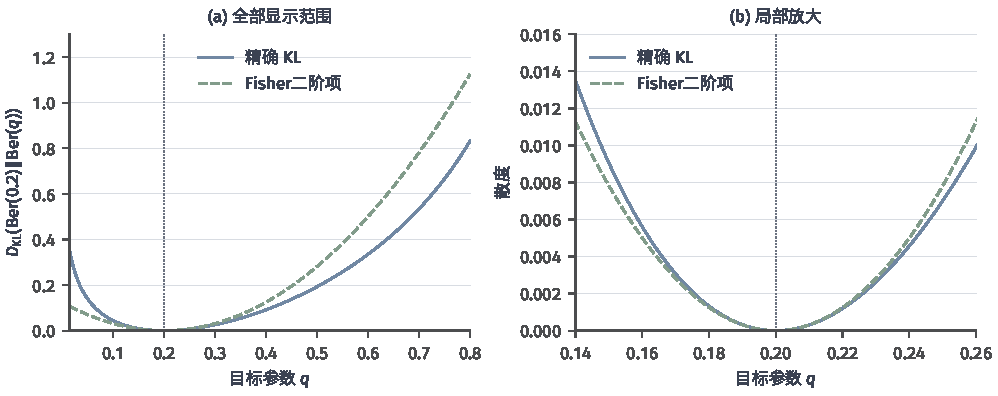
\includegraphics[width=\linewidth]{figures/00-shared/mathematical-preliminaries-lower/01-random-variables-distributions-and-causality/matplotlib/information-fisher-local/figure.pdf}
  \caption{Bernoulli族在\(p=0.2\)处的Fisher局部近似（解析式教学图）。
  蓝实线为\(D_{\mathrm{KL}}(P_{0.2}\Vert P_q)\)，绿虚线为
  \((q-0.2)^2/[2(0.2)(0.8)]\)；右图放大邻域。图中\(0<q<1\)，
  二阶式只描述足够小的参数扰动。}
  \label{fig:information-fisher-local}
\end{figure*}

\paragraph{重参数化下的几何保持}
\label{sec:information-fisher-reparameterization}

令\(\bm\theta=\bm\theta(\bm\phi)\)为光滑局部可逆坐标变换，
Jacobian为\(\bm J=\partial\bm\theta/\partial\bm\phi\)。
在对应点\(P_{\bm\phi}=P_{\bm\theta(\bm\phi)}\)是同一张分布，
不是又施加一次统计扰动。链式法则给出
\[
  \bm s_{\bm\phi}=\bm J^\top\bm s_{\bm\theta},\qquad
  \bm F_{\bm\phi}=\bm J^\top\bm F_{\bm\theta}\bm J.
\]
因切向量满足\(\mathrm d\bm\theta=\bm J\,\mathrm d\bm\phi\)，
\[
  \mathrm d\bm\phi^\top\bm F_{\bm\phi}\mathrm d\bm\phi
  =\mathrm d\bm\theta^\top\bm F_{\bm\theta}\mathrm d\bm\theta.
\]
对同一标量目标\(L\)，梯度坐标变为
\(\bm g_{\bm\phi}=\bm J^\top\bm g_{\bm\theta}\)，
因此目标微分
\(\bm g_{\bm\phi}^\top\mathrm d\bm\phi
=\bm g_{\bm\theta}^\top\mathrm d\bm\theta\)也不变。
Fisher矩阵的数值会变，不变的是它作用于对应切向量所得到的二次型。

例如Bernoulli概率\(p\)改用logit坐标\(\phi=\log[p/(1-p)]\)，
\(\mathrm dp/\mathrm d\phi=p(1-p)\)，于是
\[
  F_\phi=\{p(1-p)\}^2F_p=p(1-p).
\]
一个坐标下的Fisher在边界附近变大，另一个变小，
但对同一分布扰动，
\((\mathrm dp)^2/[p(1-p)]=p(1-p)(\mathrm d\phi)^2\)。
坐标变换退化时不在上述局部可逆范围，例如立方高斯例子在零点的Jacobian为零。

在序贯模型中，不同概率对象会给出不同的Fisher矩阵。
先把状态\(s\)视为输入、行动\(a\)视为输出，
\(\pi_{\bm\theta}(\cdot\mid s)\)就是一个参数化条件分布，
\(d\)是给输入状态加权的固定概率分布。
这里用“策略”称呼这个条件行动核；完整的行动与环境语义留给后面的决策章节。
固定状态\(s\)，策略\(\pi_{\bm\theta}(a\mid s)\)的单步Fisher为
\[
  \bm F_s(\bm\theta)
  =\mathbb E_{A\sim\pi_{\bm\theta}(\cdot\mid s)}
    [\bm s_{\bm\theta}(s,A)\bm s_{\bm\theta}(s,A)^\top].
\]
若状态访问权重\(d(s)\)被指定并保持固定，
平均矩阵为\(\bm F_d=\mathbb E_{S\sim d}\bm F_S\)。
它衡量这一输入权重下的条件策略变化。
若把\(d_{\bm\theta}(s)\pi_{\bm\theta}(a\mid s)\)作为完整联合模型求导，
得分还包含\(\nabla\log d_{\bm\theta}(s)\)。
在正则条件下，条件策略得分均值为零，交叉项消失，联合Fisher成为
\[
  \bm F_{d_{\bm\theta}\pi_{\bm\theta}}
  =\bm F_{d_{\bm\theta}}^{\mathrm{state}}
    +\mathbb E_{d_{\bm\theta}}\bm F_S.
\]
它与把当前访问权重固定后得到的平均矩阵不是同一个对象。

第三个对象是完整轨迹Fisher。设初始分布和环境转移都不依赖参数，
参数只出现在固定有限时域\(T\)的条件动作核中。
假设共同支持和交换微分成立，各步得分的二阶矩有限，即得分平方可积。
轨迹得分为\(\sum_{t=1}^T\bm s_t\)，其中
\(\mathbb E[\bm s_t\mid H_t]=\bm0\)，\(H_t\)为选择动作前的历史。
当\(u<t\)时，\(\bm s_u\)对\(H_t\)可测，因此
\[
  \mathbb E[\bm s_u\bm s_t^\top]
  =\mathbb E[\bm s_u\,\mathbb E(\bm s_t^\top\mid H_t)]=\bm0.
\]
展开外积便得到
\[
  \bm F_{\mathrm{trajectory}}
  =\sum_{t=1}^T\mathbb E[\bm F_{H_t}],
\]
而不是某个任意固定访问分布下的单步矩阵。
Markov策略下可把条件矩阵写成\(\bm F_{S_t}\)；
若访问权重取各时刻边缘的平均，轨迹矩阵等于对应平均矩阵的\(T\)倍。
环境或初始规律也含参数时，必须加入它们的得分，不能沿用策略独占参数的公式。

另一个常见混淆发生在样本矩阵与模型期望之间。
固定输入分布\(d\)，取条件高斯
\(Y\mid\bm X=\bm x\sim\mathcal N(\bm\theta^\top\bm x,\sigma^2)\)，
其中\(\sigma>0\)已知，\(\mathbb E_d\|\bm X\|^2<\infty\)。
同一观测的三个量为
\[
\begin{aligned}
  \bm s_{\bm\theta}(\bm x,y)
    &=\frac{y-\bm\theta^\top\bm x}{\sigma^2}\bm x,\\
  -\nabla^2_{\bm\theta}\log p_{\bm\theta}(y\mid\bm x)
    &=\frac{\bm x\bm x^\top}{\sigma^2},\\
  \bm s_{\bm\theta}\bm s_{\bm\theta}^\top
    &=\frac{(y-\bm\theta^\top\bm x)^2}{\sigma^4}\bm x\bm x^\top.
\end{aligned}
\]
按当前模型的条件分布平均时，残差平方期望为\(\sigma^2\)，
后两个矩阵的条件期望相同，再按\(d\)平均得到
\(\bm F=\mathbb E_d[\bm X\bm X^\top]/\sigma^2\)。
对一条样本，它们并不相等；残差为零时，得分外积甚至为零，
而非零输入的观测Hessian不为零。
如果真实响应规律不同于当前模型，残差平方的条件期望也可能不同，
经验得分外积的总体极限便不一定等于这个模型Fisher。
改变输入权重、使用观测Hessian或经验得分外积，都须重新说明正在近似哪个对象。

\subsection{基于分布几何的参数更新}
\label{sec:information-geometric-update}

局部Fisher度量把参数方向的长度与相应的分布变化联系起来。固定参数点后，对目标作一阶线性化、对KL作二阶近似，就能在给定二次长度预算内选择下降最多的方向，这导出负自然梯度。这个“最多”针对局部近似子问题，不声称任意有限步更新都解出了精确KL约束下的原优化问题。
这仍是原优化任务的局部求解步骤：若参数表示有约束，应在相应可行切空间中求解，
或结合约束优化和回缩；Fisher矩阵本身不会自动保持矩与固定边缘。

\paragraph{分布变化约束下的自然梯度}
\label{sec:information-natural-gradient-update}

设目标\(L(\bm\theta)\)可微，\(\bm g=\nabla L(\bm\theta)\)，
且\(\bm F(\bm\theta)\)正定。欧氏梯度是目标微分在欧氏内积下的代表；
改用Fisher内积，代表向量也应随之改变\scite{math-amari1998natural}
\begin{definition}[自然梯度]
\label{def:information-natural-gradient}
目标\(L\)的\term{自然梯度}（natural gradient）是满足
\[
  g_{\bm\theta}(\operatorname{grad}^{F}L,\bm v)
  =\nabla L(\bm\theta)^\top\bm v
  \quad\text{对所有切向量 }\bm v
\]
的唯一向量，即
\(\operatorname{grad}^{F}L=\bm F(\bm\theta)^{-1}\nabla L(\bm\theta)\)。
\end{definition}

把目标一阶线性化，把分布KL变化二阶近似，得到局部信赖域子问题
\begin{equation}
  \min_{\bm\delta}\bm g^\top\bm\delta
  \quad\text{s.t.}\quad
  \tfrac12\bm\delta^\top\bm F(\bm\theta)\bm\delta\leq\varepsilon.
  \label{eq:information-natural-gradient-trust-region}
\end{equation}
设\(\varepsilon>0,\bm g\neq\bm0\)。
Lagrangian为
\(\bm g^\top\bm\delta+\lambda(\bm\delta^\top\bm F\bm\delta/2-\varepsilon)\)，
驻点条件给出
\(\bm g+\lambda\bm F\bm\delta=\bm0\)。
非零线性目标的最小值在椭球边界，
代入\(\bm\delta=-\lambda^{-1}\bm F^{-1}\bm g\)得到
\(\lambda=\sqrt{\bm g^\top\bm F^{-1}\bm g/(2\varepsilon)}\)，所以
\begin{equation}
  \bm\delta^\star
  =-\sqrt{\frac{2\varepsilon}{\bm g^\top\bm F^{-1}\bm g}}\,
    \bm F^{-1}\bm g.
  \label{eq:information-natural-gradient-step}
\end{equation}

可以不依赖驻点必要条件，直接验证全局最优性。
令\(\bm u=\bm F^{1/2}\bm\delta\)，约束变为
\(\|\bm u\|_2\leq\sqrt{2\varepsilon}\)，目标变为
\((\bm F^{-1/2}\bm g)^\top\bm u\)。
Cauchy--Schwarz给出
\[
  (\bm F^{-1/2}\bm g)^\top\bm u
  \geq-\|\bm F^{-1/2}\bm g\|_2\sqrt{2\varepsilon}.
\]
等号在\(\bm u\)与\(-\bm F^{-1/2}\bm g\)同向并位于球面时达到，
代回正好得到上述解。若\(\bm g=\bm0\)，一阶目标处处为零，
子问题不再选出唯一方向，应考察高阶信息或停止条件。

\begin{example}[同一分布变化预算下的两个下降方向]
\label{ex:information-natural-gradient-ellipse}
设在当前参数点，局部Fisher矩阵与目标梯度为
\[
 \bm F=\begin{pmatrix}100&0\\0&1\end{pmatrix},
 \qquad \bm g=\begin{pmatrix}1\\1\end{pmatrix}.
\]
目标的一阶变化为\(\delta_1+\delta_2\)，但同样大小的第一维位移消耗的二次KL预算
是第二维的\(100\)倍。取局部预算\(\varepsilon=0.005\)，可行椭圆为
\(100\delta_1^2+\delta_2^2\leq0.01\)。普通欧氏下降方向是\(-\bm g\)，
自然下降方向是\(-\bm F^{-1}\bm g=-(0.01,1)^\top\)。
为公平比较，把两个方向都缩放到同一椭圆边界，得到
\[
 \bm\delta_{\mathrm E}=-\frac{0.1}{\sqrt{101}}(1,1)^\top,
 \qquad
 \bm\delta_{\mathrm F}=-\frac{0.1}{\sqrt{1.01}}(0.01,1)^\top.
\]
两者都恰好消耗\(0.005\)的二次预算，目标的一阶下降量分别为
\[
 -\bm g^\top\bm\delta_{\mathrm E}
 =\frac{0.2}{\sqrt{101}}\approx0.0199,
 \qquad
 -\bm g^\top\bm\delta_{\mathrm F}
 =0.1\sqrt{1.01}\approx0.1005.
\]
自然方向减少昂贵的第一维移动，把更多预算用于第二维，因此在当前局部模型中获得
更大的下降量。这里\(\bm F\)刻画分布变化的局部代价，不是一般目标\(L\)的Hessian；
上述数值比较的是线性化目标与二次KL模型，不能直接当作真实目标的有限步下降保证。
\end{example}

图~\ref{fig:information-natural-gradient-ellipse}把两个缩放后的方向放在同一预算边界上。
两轴采用相同的物理尺度，细长椭圆说明第一维允许的位移更小。
\begin{figure}[htbp]
  \centering
  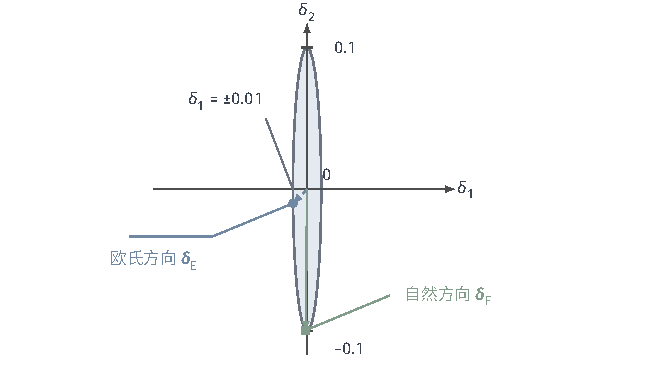
\includegraphics[width=\linewidth]{figures/00-shared/mathematical-preliminaries-lower/01-random-variables-distributions-and-causality/tikz/information-natural-gradient-ellipse/figure.pdf}
  \caption{局部KL预算下的下降方向（解析式教学图）。灰色椭圆满足
  \(100\delta_1^2+\delta_2^2=0.01\)，对应\(\varepsilon=0.005\)。
  蓝色虚线与圆点是缩放后的欧氏方向\(\bm\delta_{\mathrm E}\)，绿色实线与方点是
  自然方向\(\bm\delta_{\mathrm F}\)；两个终点消耗相同的二次预算。
  椭圆表达分布变化代价，不是目标函数的等高线。}
  \label{fig:information-natural-gradient-ellipse}
\end{figure}

在光滑可逆重参数化下，由上一小节的矩阵和微分变换，
\[
\begin{aligned}
  \bm J\bm F_{\bm\phi}^{-1}\bm g_{\bm\phi}
  &=\bm J(\bm J^\top\bm F_{\bm\theta}\bm J)^{-1}
    \bm J^\top\bm g_{\bm\theta}\\
  &=\bm F_{\bm\theta}^{-1}\bm g_{\bm\theta}.
\end{aligned}
\]
归一化因子中的
\(\bm g_{\bm\phi}^\top\bm F_{\bm\phi}^{-1}\bm g_{\bm\phi}\)
也等于原坐标下的相应值，因此两个坐标给出同一个分布切向方向。
Bernoulli例子中，自然梯度在概率坐标为\(p(1-p)L'(p)\)，
在logit坐标为\(L'(p)\)；乘上\(\mathrm dp/\mathrm d\phi=p(1-p)\)后相同。

保持的是无穷小方向，不是任意有限离散步。
非线性坐标映射下，
\(\bm\theta(\bm\phi+\bm\delta_\phi)
=\bm\theta(\bm\phi)+\bm J\bm\delta_\phi+O(\|\bm\delta_\phi\|^2)\)，
所以分别做欧氏加法更新后的终点一般不同。
真实KL也还有\(o(\|\bm\delta\|^2)\)余项；
二次预算等于\(\varepsilon\)不保证真实KL严格不超过它。
有限步需要步长选择、真实目标或KL检查，不能由局部方向不变性直接得到全局改进。

\paragraph{奇异与近似条件下的几何更新}
\label{sec:information-singular-approximate-update}

参数冗余、退化坐标或不足的输入方向都可能使Fisher奇异。
其零空间只说明相应方向的一阶得分为零：
有时它来自完全冗余，有时如立方高斯零点，只是高阶变化未被二次型看见。
因而不能把所有零方向都理解成有限移动后分布完全不变。

回用伪逆与数值求解工具，若\(\bm g\in\operatorname{range}(\bm F)\)，
线性方程\(\bm F\bm v=\bm g\)有解，全部解为
\[
  \bm v=\bm F^\dagger\bm g+\bm z,\qquad
  \bm z\in\ker\bm F.
\]
伪逆选择当前欧氏坐标下范数最小的一个。
在得分能识别的切向商空间中，零空间分量不影响一阶分布方向，
但参数向量并不唯一，有限步的高阶效果仍可能不同。
若\(\bm g\notin\operatorname{range}(\bm F)\)，存在零方向
\(\bm z\)使\(\bm g^\top\bm z\neq0\)；
沿其下降方向任意放大仍不消耗二次预算，线性信赖域问题无下界。
此时简单写\(\bm F^\dagger\bm g\)不是原信赖域子问题的解，必须修正退化模型或约束。

阻尼使用\(\bm F+\lambda\bm I\)，其中\(\lambda>0\)，可改善病态性并保证可逆。
但它新增欧氏二次项\(\lambda\|\bm\delta\|^2\)，不是纯粹的Fisher几何：
一般坐标变化下
\[
  \bm J^\top(\bm F+\lambda\bm I)\bm J
  =\bm J^\top\bm F\bm J+\lambda\bm J^\top\bm J
  \neq\bm F_{\bm\phi}+\lambda\bm I.
\]
因此“能稳定求逆”与“保持原坐标变换性质”是不同要求。
实际计算通常求解线性系统，而不显式构造逆矩阵；
迭代容差、谱条件和矩阵近似误差也会改变得到的方向。

经验Fisher、分块或对角近似可能降低计算量，
却分别引入抽样、模型期望或跨块相关性的近似。
即使每个近似矩阵都正定，也只说明定义了某种局部内积，
不说明它等于真实分布Fisher，更不保证同样的坐标保持结论。
应区分模型下期望、真实观测分布下平均、固定预测特征的权重和完整轨迹，
再说明哪一项被估计或省略。
优化收敛、模型正确性、预测校准和隐私保证还各有自己的条件；
自然梯度或KL正则不能把一种保证自动转成另一种。

\section{本章小结}
\label{sec:information-theory-statistical-geometry-summary}

同一组概率规律可以回答不同问题，比较时应先确定保留的对象。熵给出已知规律下的平均自信息，无失真编码还须满足前缀、整数码长与共享模型约束；连续记录离不开指定精度，微分熵也随参考测度及坐标改变。允许近似还原后，量化失真与码率需要共同报告，率失真函数给出明确源模型、失真准则与渐近编码范围下的极限。

分布差异的尺度决定哪些变化被看见。TV控制事件概率，核均值比较指定特征的平均，Wasserstein计入质量搬运的几何，对数密度比则给出KL与R\'enyi散度。信息、距离、核与网格都能在各自条件下度量依赖，但总体零值的识别不等于有限样本检验已经可靠。弱收敛保留有界连续探针；无界成本还需要尾部条件，不能只看概率质量是否接近。

这些关系进一步约束分布优化。期望响应的界必须与评价函数的值域、敏感性或指数矩相匹配。Gibbs倾斜、最大熵、表示受限的变分逼近与边缘受限的最优耦合，分别改变不同的可行集合；存在最优分布与能够用有限参数或有限计算实现它，也需要分别核对。Fisher信息把正则参数变化下的局部KL写成二次型，自然梯度据此选择分布步长，其坐标不变性仍依赖可识别性、正则条件与所用的近似。

本章建立的是已知规律下的描述、比较与优化依据。下一章把这些规律组成随机序列和路径，研究历史依赖、累计偏差与极限；随后统计推断再讨论只有有限观测时怎样估计未知规律，以及这些结论能获得何种误差与下界保证。
